% \begin{savequote}[8cm]
% \textlatin{Cor animalium, fundamentum e\longs t vitæ, princeps omnium, Microco\longs mi Sol, a quo omnis vegetatio dependet, vigor omnis \& robur emanat.}

% The heart of animals is the foundation of their life, the sovereign of everything within them, the sun of their microcosm, that upon which all growth depends, from which all power proceeds.
%   \qauthor{--- William Harvey \cite{harvey_exercitatio_1628}}
% \end{savequote}

\chapter{\label{app:figures}Reference Figures and Tables}

\minitoc

\section{Sample Explanations from Chapter \ref{ch:xai}}\label{app:xaifigures}

\begin{figure}[!htbp]
    \centering
    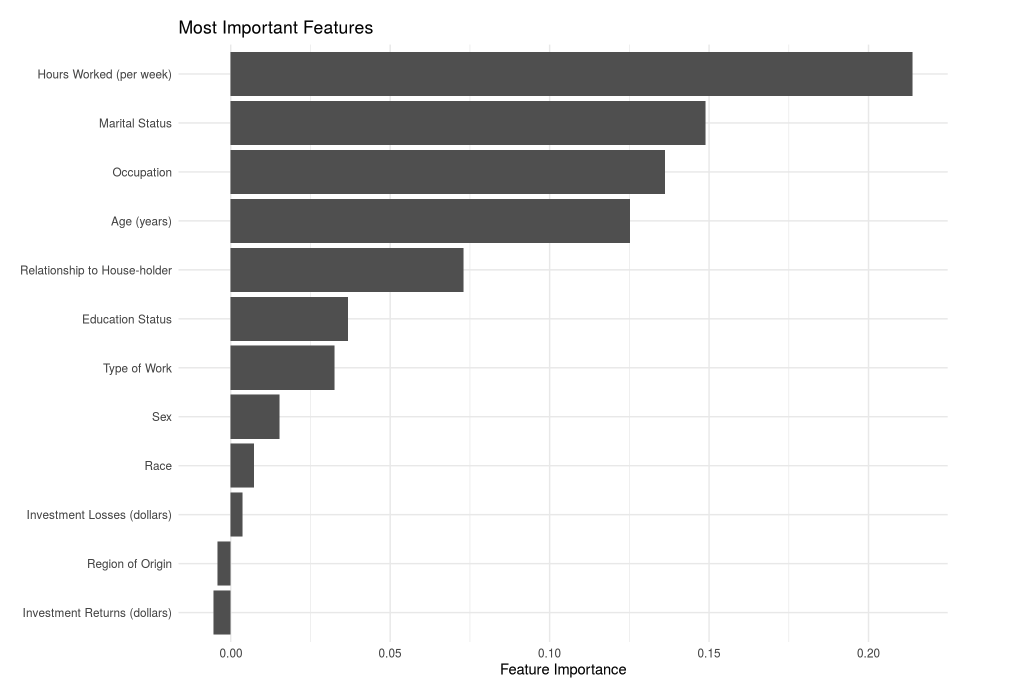
\includegraphics[width=0.9\linewidth]{xai/survey-shap.png}
    \caption{This figure shows sample SHAP explanations in the \emph{Salary} task. Features can be seen along the y-axis, while feature importance is shown based on direction and magnitude of the associated bar.}
    \label{fig:shapsalaryfull}
\end{figure}

\begin{figure}[!hbtp]
    \centering
    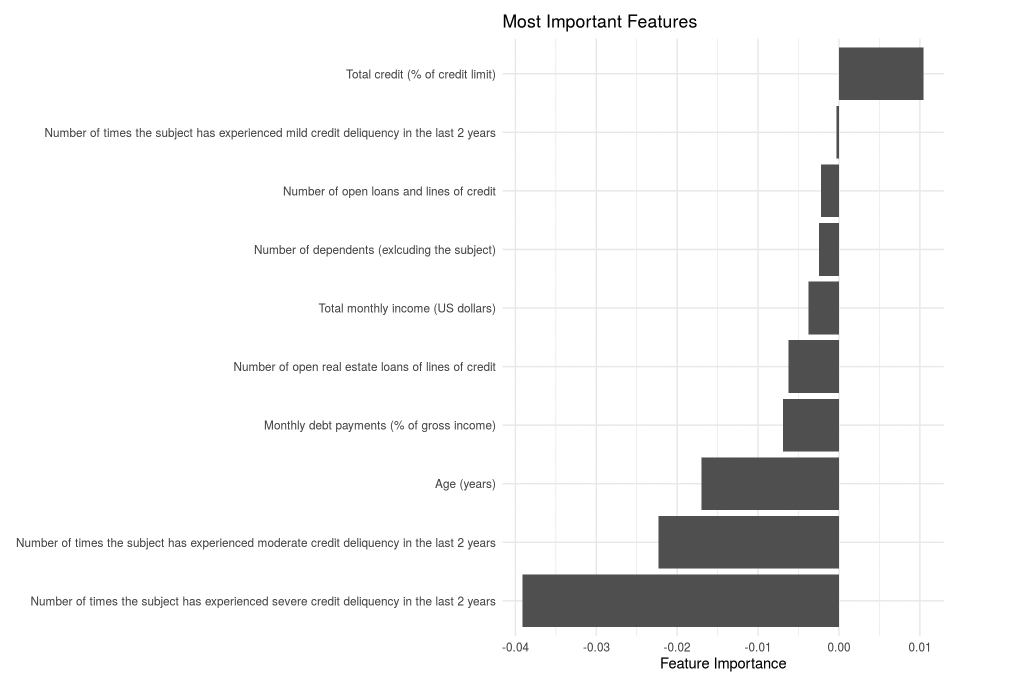
\includegraphics[width=0.9\linewidth]{xai/survey-shap-2.png}
    \caption{This figure shows sample SHAP explanations in the \emph{Credit} task. Features can be seen along the y-axis, while feature importance is shown based on direction and magnitude of the associated bar.}
    \label{fig:shapcreditfull}
\end{figure}

\begin{figure}[!hbtp]
    \centering
    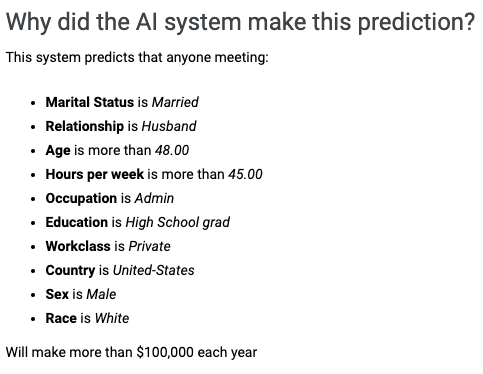
\includegraphics[width=0.8\linewidth]{xai/survey-anchor.png}
    \caption{This figure shows sample Anchor explanations in the \emph{Salary} task. The explanation shows a set of rules that, when jointly followed, increases the likelihood that the model will yield the displayed prediction.}
    \label{fig:anchorsalaryfull}
\end{figure}

\begin{figure}[!hbtp]
    \centering
    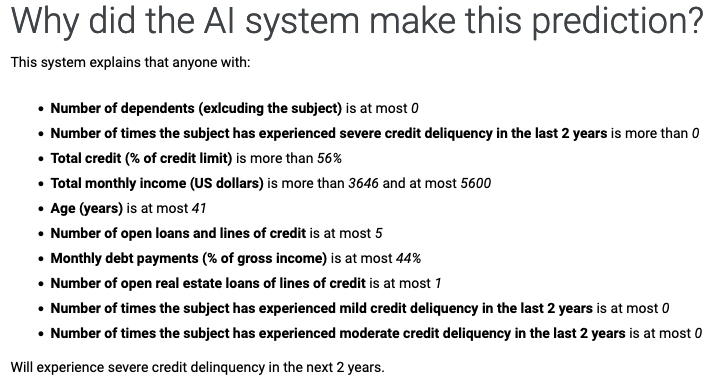
\includegraphics[width=0.9\linewidth]{xai/survey-anchor-2.png}
    \caption{This figure shows sample Anchor explanations in the \emph{Credit} task. The explanation shows a set of rules that, when jointly followed, increases the likelihood that the model will yield the displayed prediction.}
    \label{fig:anchorcreditfull}
\end{figure}

\begin{figure}[!hbtp]
    \centering
    
\includegraphics[width=0.6\linewidth]{xai/survey-confidence.png}
    \caption{This figure shows sample Confidence explanations in the \emph{Salary} task. The explanation is simply one sentence containing the model's confidence parameter.}
    \label{fig:confidencesalaryfull}
\end{figure}

\begin{figure}[!hbtp]
    \centering
    
\includegraphics[width=0.6\linewidth]{xai/survey-confidence-2.png}
    \caption{This figure shows sample Confidence explanations in the \emph{Credit} task. The explanation is simply one sentence containing the model's confidence parameter.}
    \label{fig:confidencecreditfull}
\end{figure}

\newpage
\section{Images and Descriptions of Prototypes from Chapter \ref{ch:diversity}}\label{app:divfigures}

\begin{figure}[!hbtp]
    \centering
    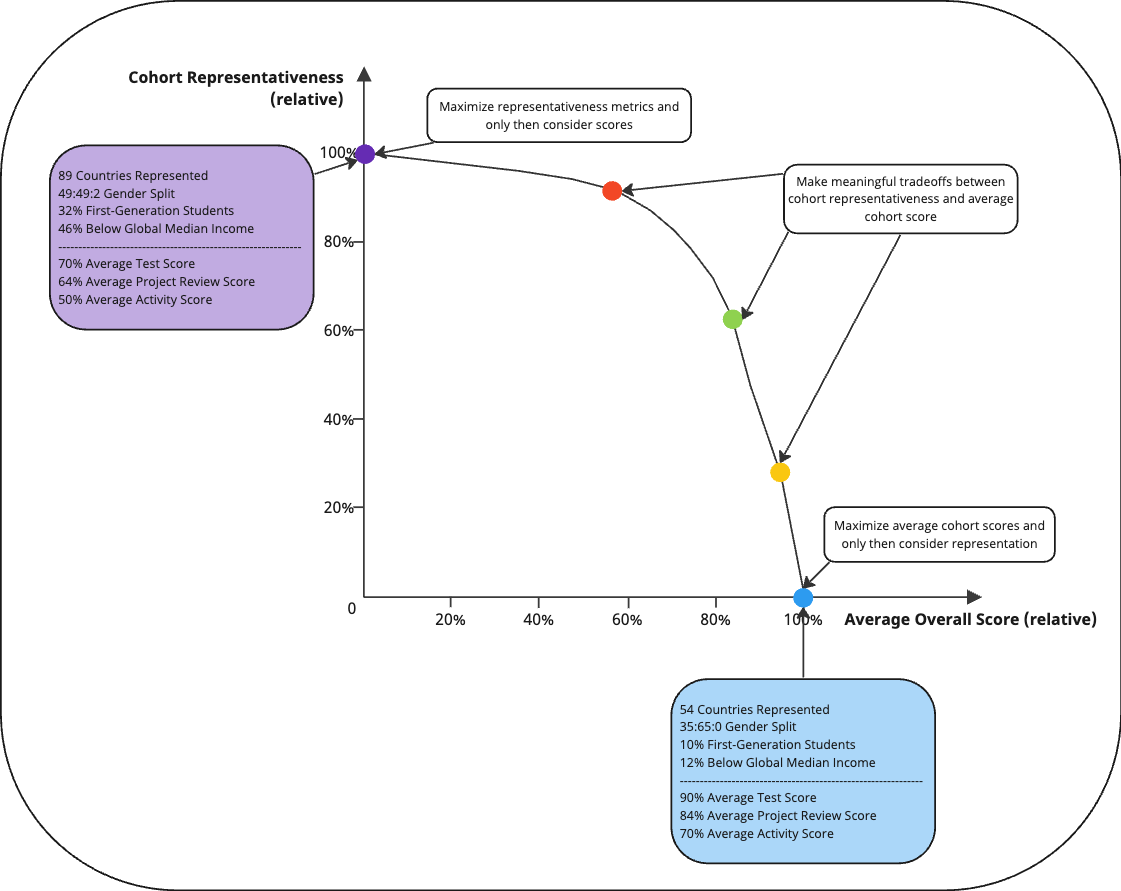
\includegraphics[width=0.9\linewidth]{diversity/representativeness.png}
    \caption{This figure reproduces Prototype \ref{fig:representativeness} at a larger scale.}
    \label{fig:representativeness_full}
\end{figure}

\begin{figure}[!hbtp]
    \centering
    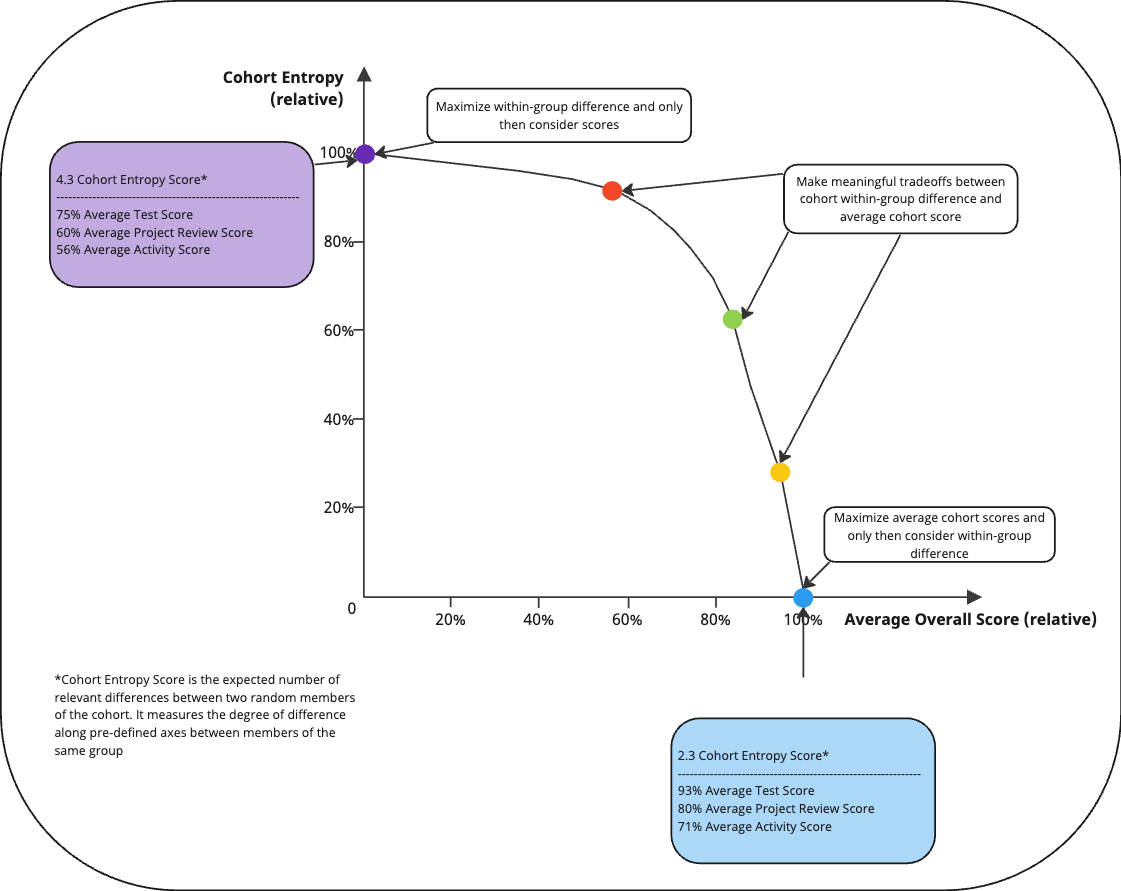
\includegraphics[width=0.9\linewidth]{diversity/entropy.png}
    \caption{This figure reproduces Prototype \ref{fig:entropy} at a larger scale.}
    \label{fig:entropy_full}
\end{figure}

\begin{figure}[!hbtp]
    \centering
    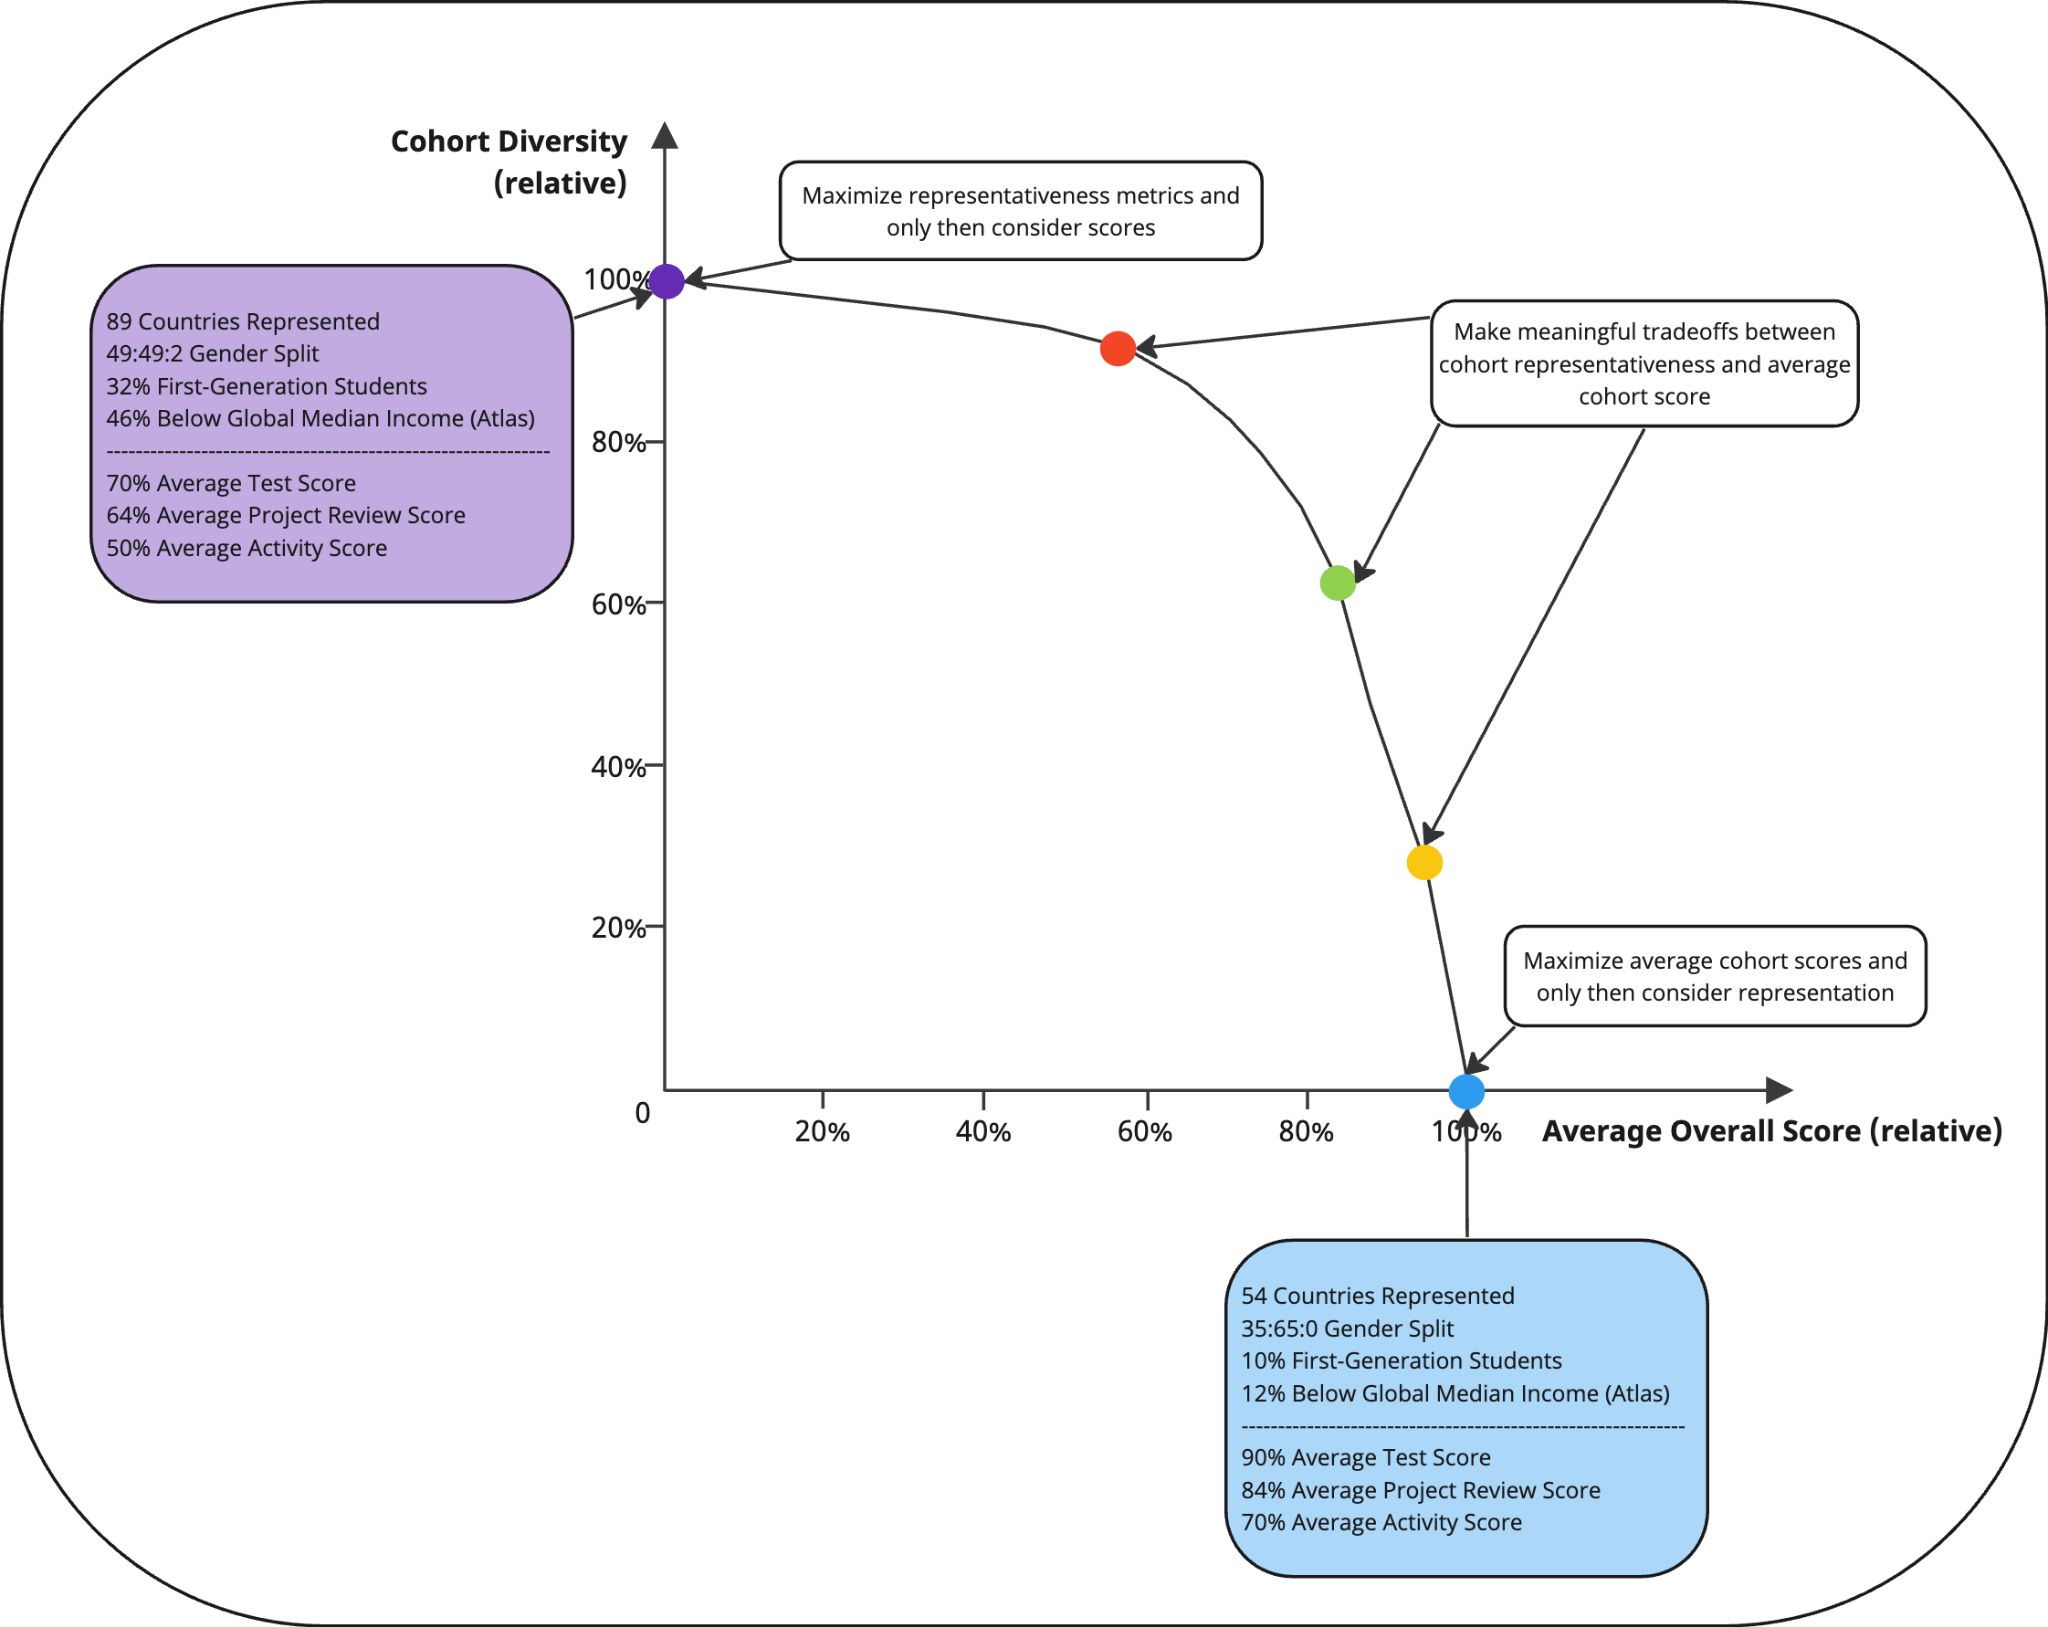
\includegraphics[width=0.9\linewidth]{diversity/diversity.png}
    \caption{This figure reproduces Prototype \ref{fig:diversity} at a larger scale.}
    \label{fig:diversity_full}
\end{figure}

\begin{figure}[!hbtp]
    \centering
    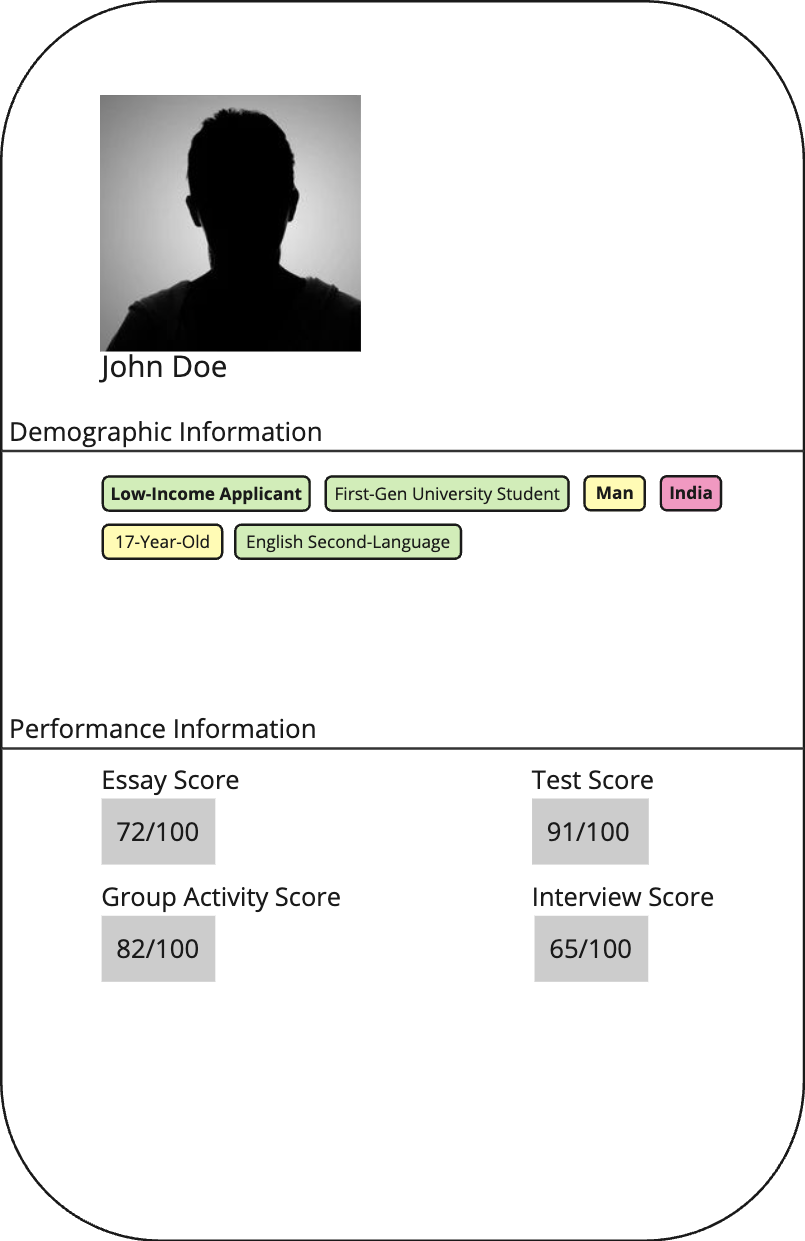
\includegraphics[width=0.9\linewidth]{diversity/demographic.png}
    \caption{This figure reproduces Prototype \ref{fig:demographic} at a larger scale.}
    \label{fig:demographic_full}
\end{figure}

\begin{figure}[!hbtp]
    \centering
    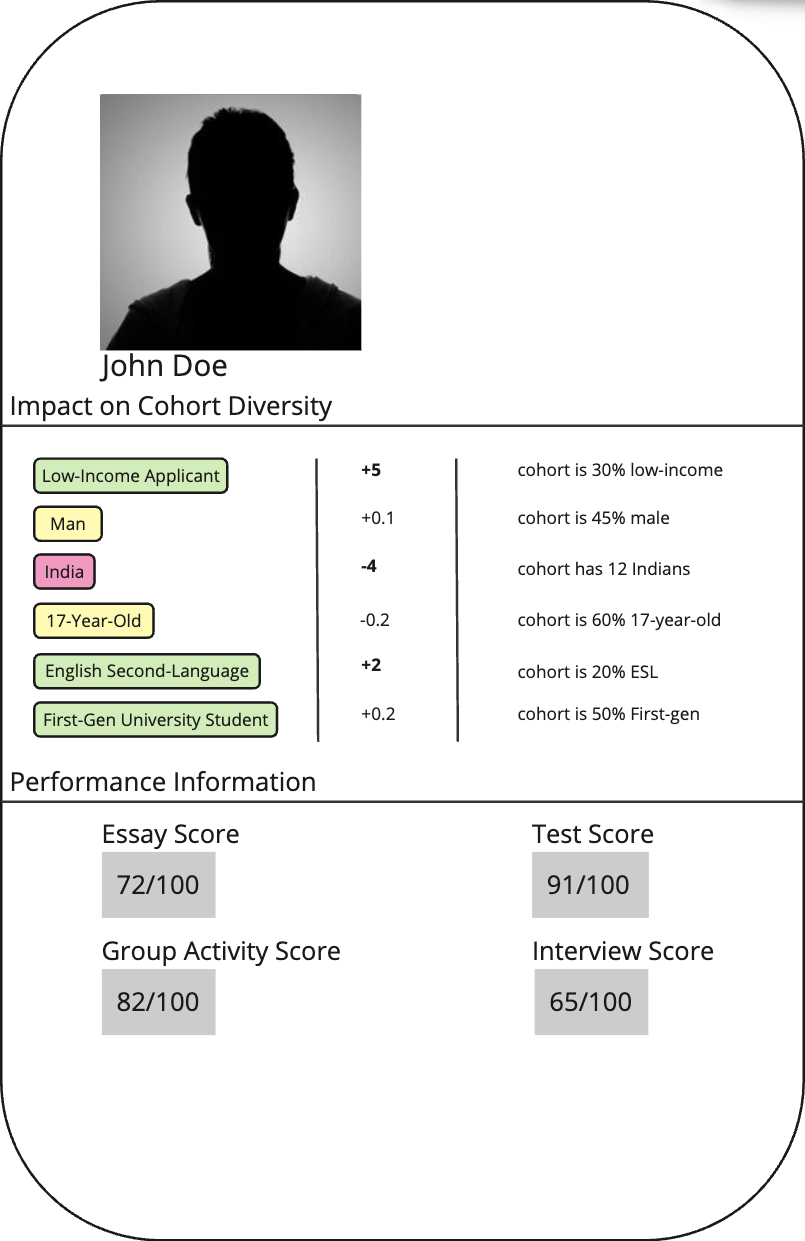
\includegraphics[width=0.9\linewidth]{diversity/impact.png}
    \caption{This figure reproduces Prototype \ref{fig:impact} at a larger scale.}
    \label{fig:impact_full}
\end{figure}

\begin{figure}[!hbtp]
    \centering
    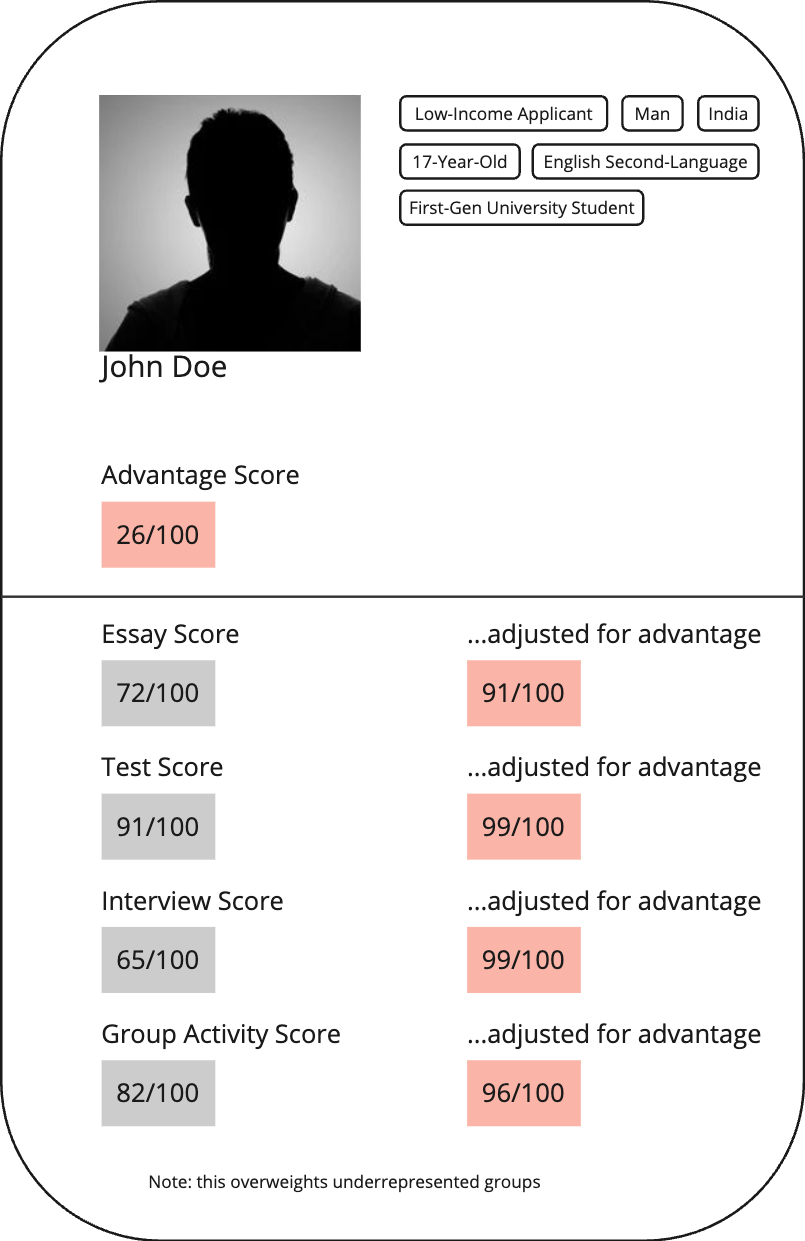
\includegraphics[width=0.9\linewidth]{diversity/advantage.png}
    \caption{This figure reproduces Prototype \ref{fig:advantage} at a larger scale.}
    \label{fig:advantage_full}
\end{figure}

\newpage
\section{Figures and Tables for Chapter \ref{ch:spf}}\label{app:spffigures}
\begin{figure}[!hbtp]
    \centering
    \label{fig:spf_2021_full}
    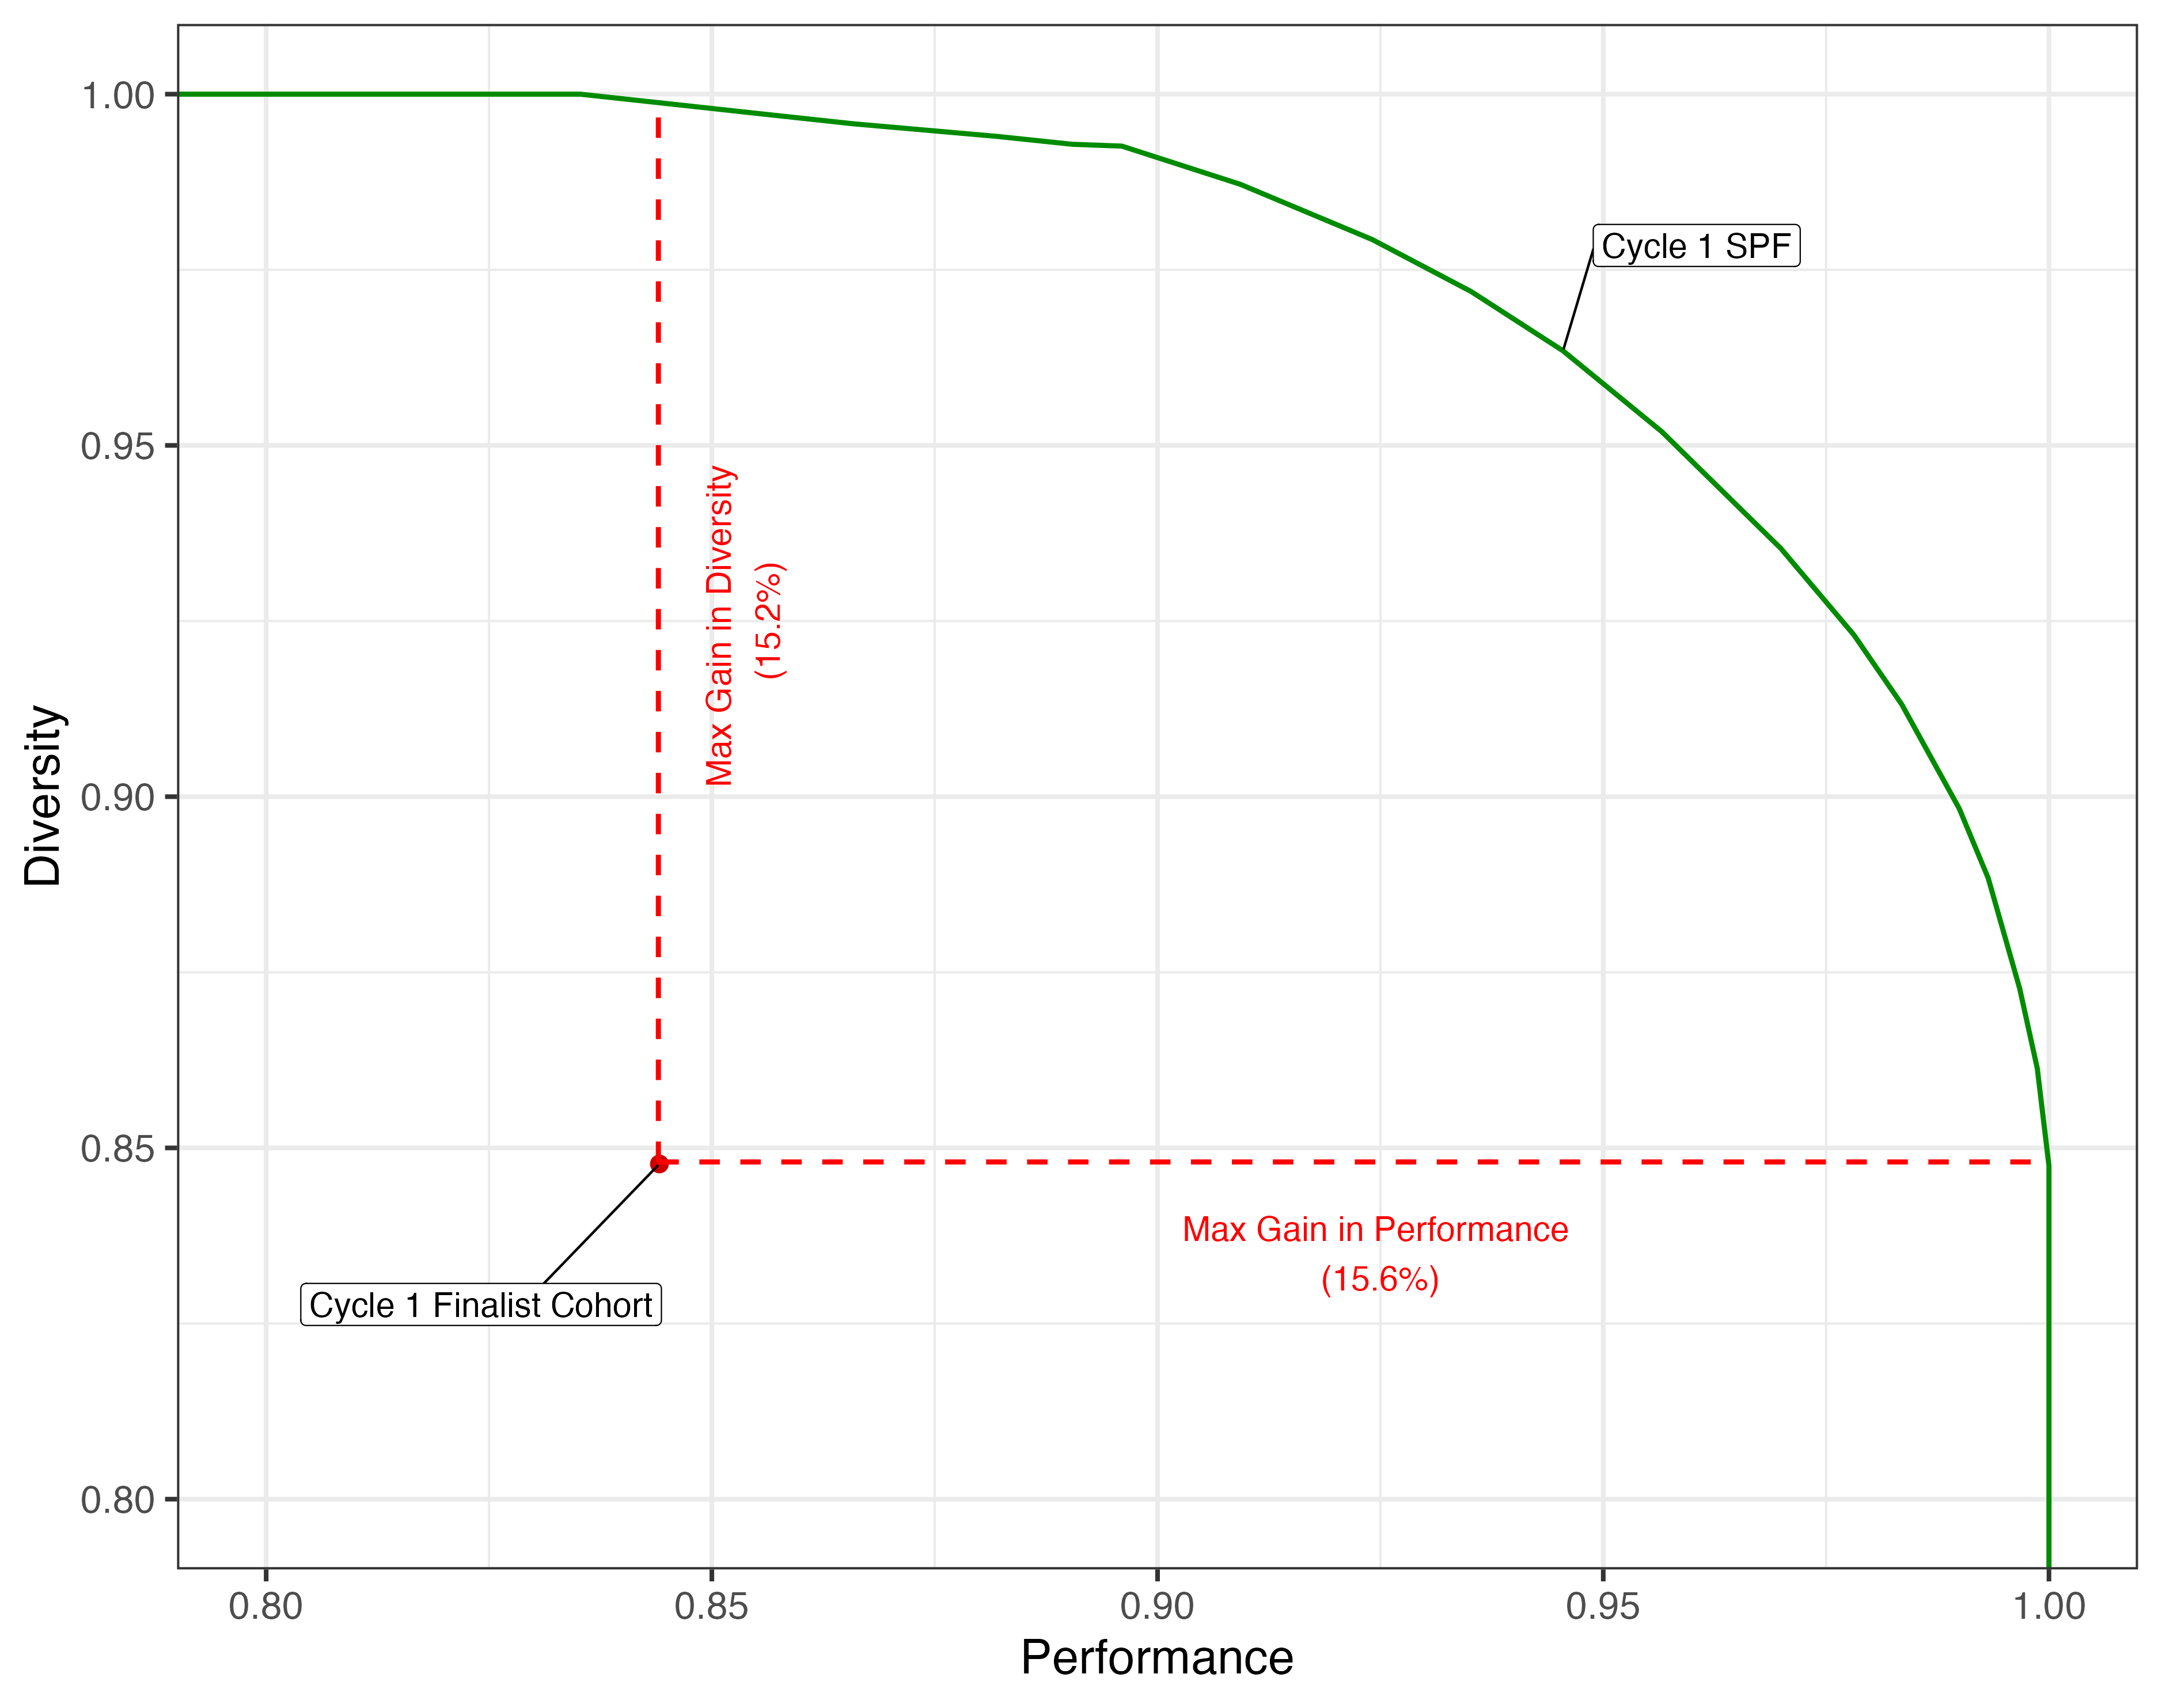
\includegraphics[width=0.9\linewidth]{spf/yr1_spf_finalist.png} 
    \caption{This figure displays the SPF we estimate for the Cycle 2021 finalist selection process. The y-axis represents the diversity score while the x-axis represents average cohort performance. The green curve is our estimate of the SPF, which represents the upper bound of diversity that is achievable at every level of cohort performance. The red dot depicts the actual level of diversity and performance of the finalists that were selected in Cycle 2021. The vertical and horizontal dashed red lines represent the maximum Pareto gain that was possible along the diversity and performance dimensions respectively. In particular, cohort diversity could have been improved by $15.2\%$ without any reduction in cohort performance. And, cohort performance could have been improved by $15.6\%$ without any cost to diversity.}
\end{figure}
    
\begin{figure}[!hbtp]
    \centering
    \label{fig:spf_2022_full}
    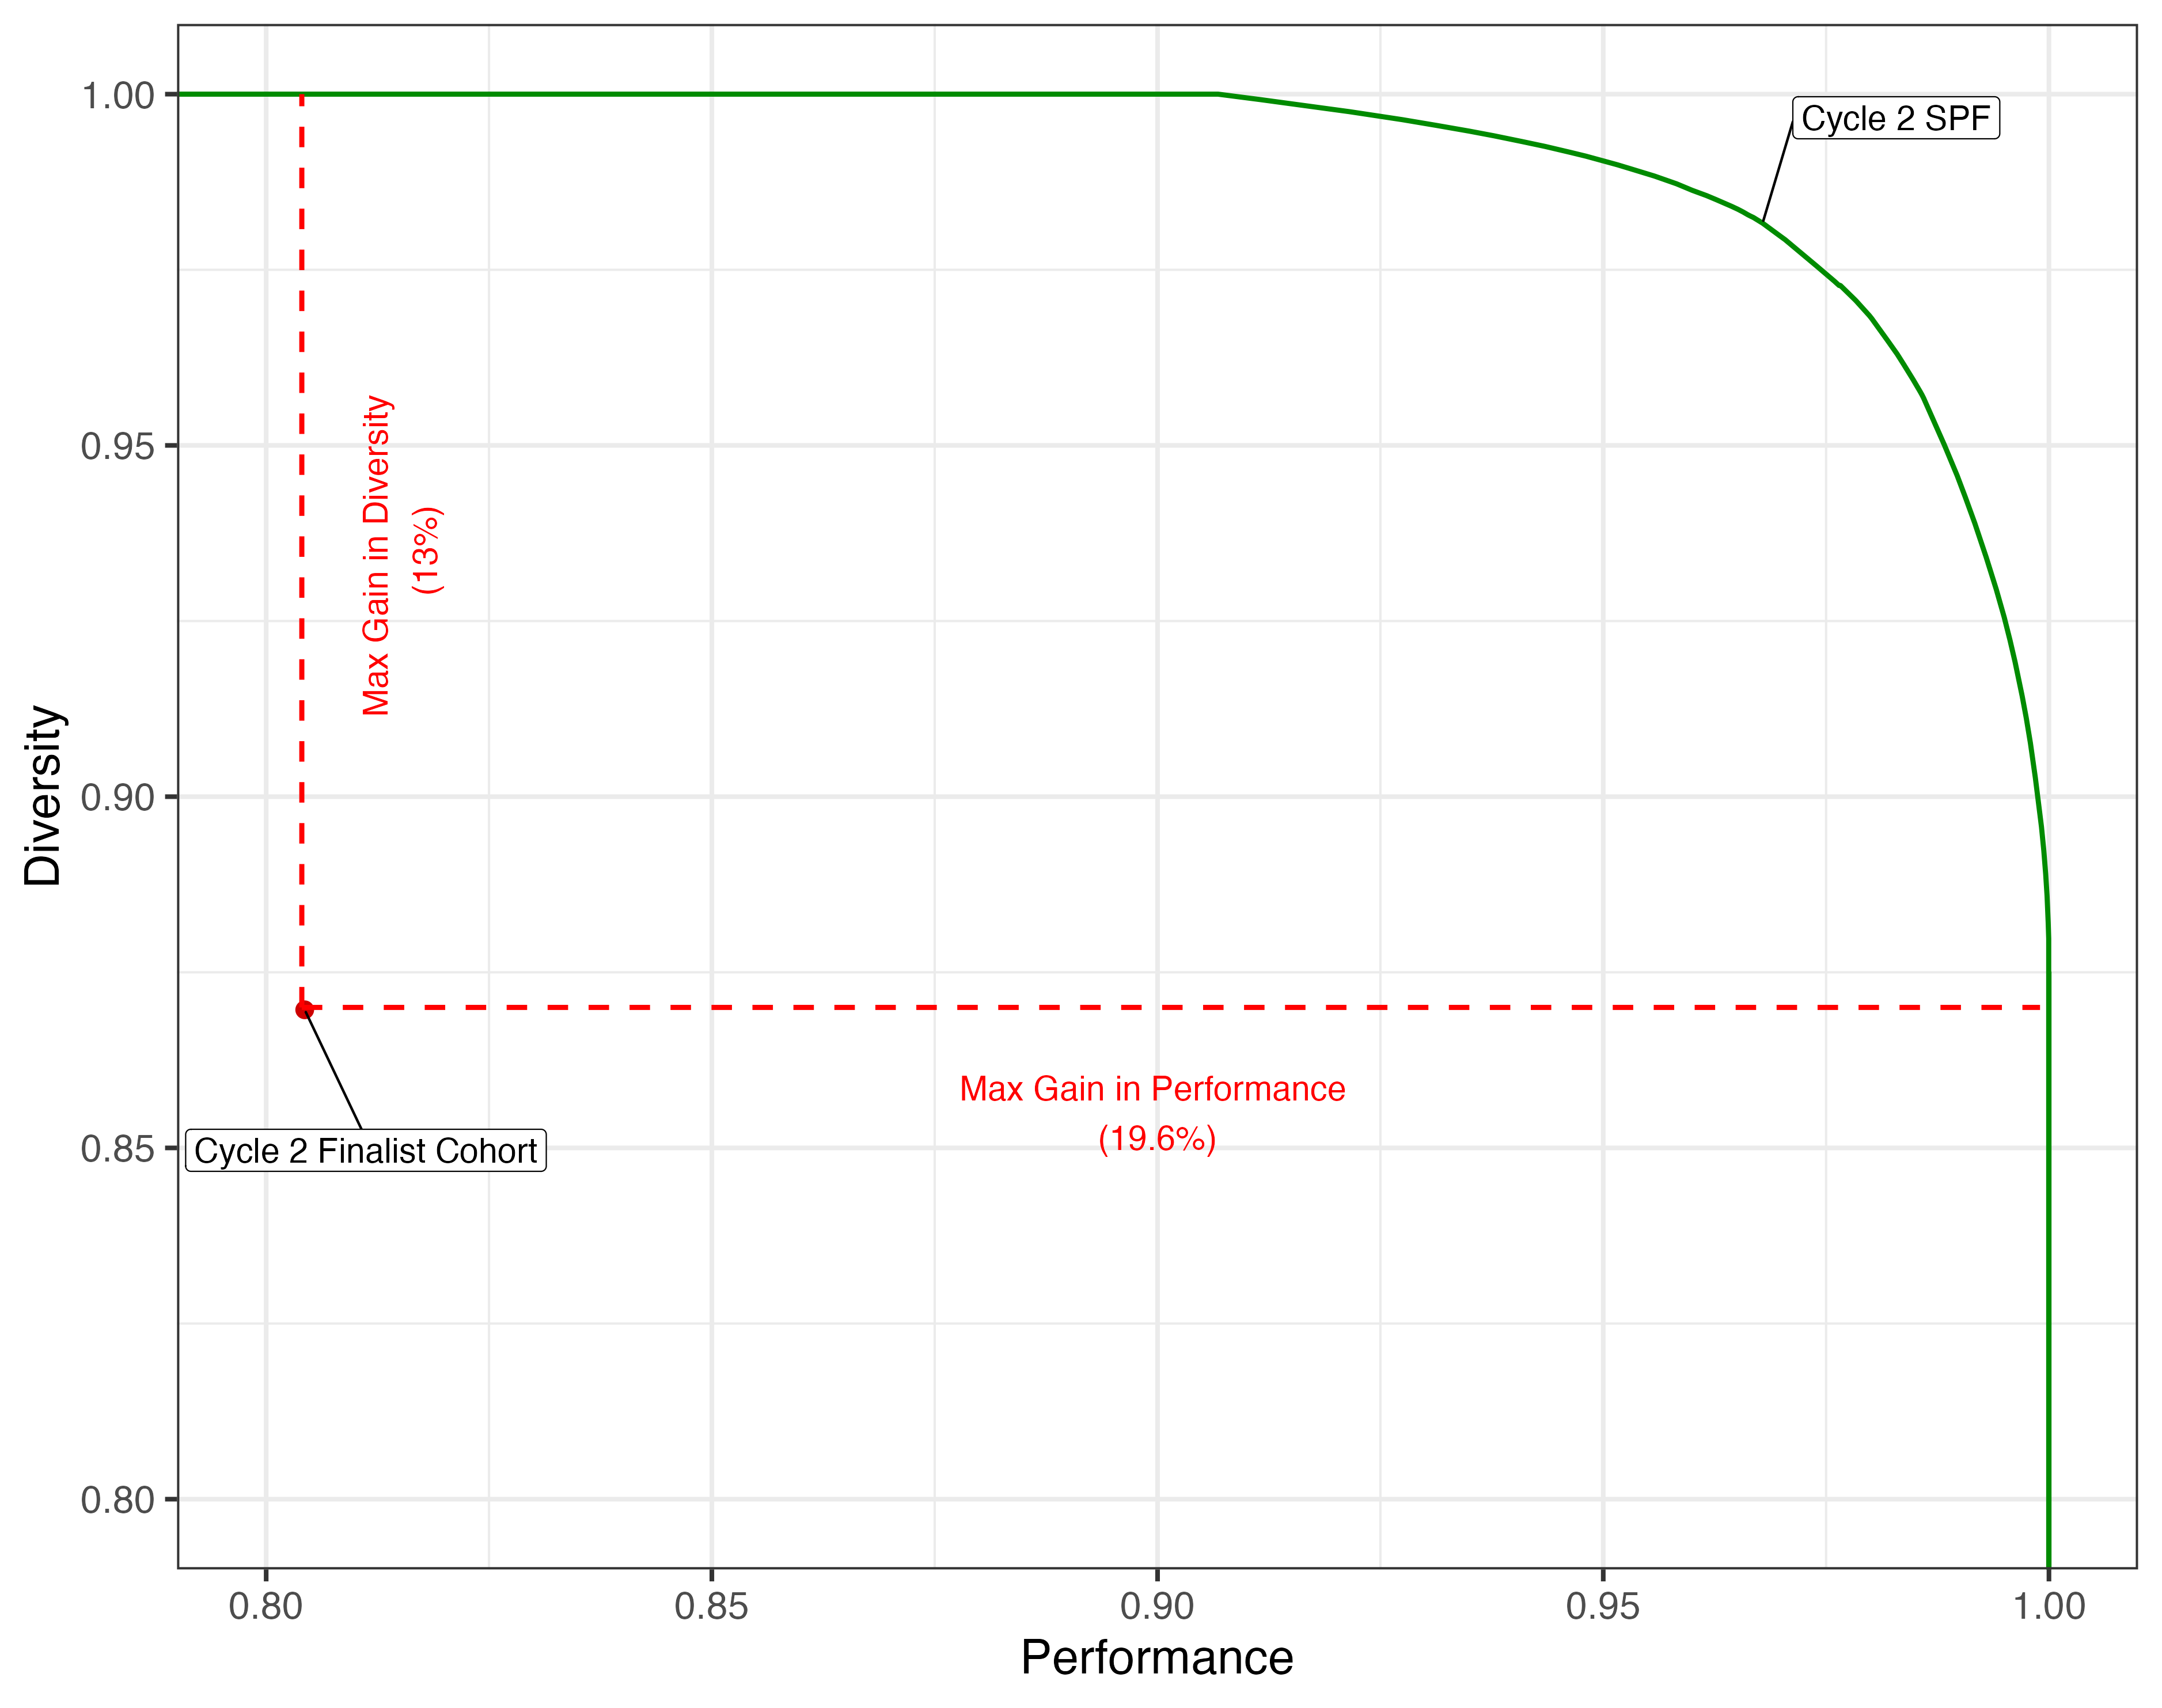
\includegraphics[width=0.9\linewidth]{spf/yr2_spf_finalist.png} 
    \caption{This figure displays the SPF we estimate for the Cycle 2022 finalist selection process. The y-axis represents the diversity score while the x-axis represents average cohort performance. The green curve is our estimate of the SPF, which represents the upper bound of diversity that is achievable at every level of cohort performance. The red dot depicts the actual level of diversity and performance of the finalists that were selected in Cycle 2022. The vertical and horizontal dashed red lines represent the maximum Pareto gain that was possible along the diversity and performance dimensions respectively. In particular, cohort diversity could have been improved by $13\%$ without any reduction in cohort performance. And, cohort performance could have been improved by $19.6\%$ without any cost to diversity.}
\end{figure}



    % \begin{figure}[!htb]
    % \centering
    %     \caption{Distribution of Cycle 1 Applicant Countries (Top 5 Labeled). Data come from surveys completed by applicants. Data are solely from the cycle 1 application cohort. Overall applicants come from 105 different countries. The distribution of proportions of applicants by country in this figure are limited to the 50 countries from which there were the most applicants. The top 5 countries are labeled on the figure. }\label{fig:dist_countryies_c1}
    %   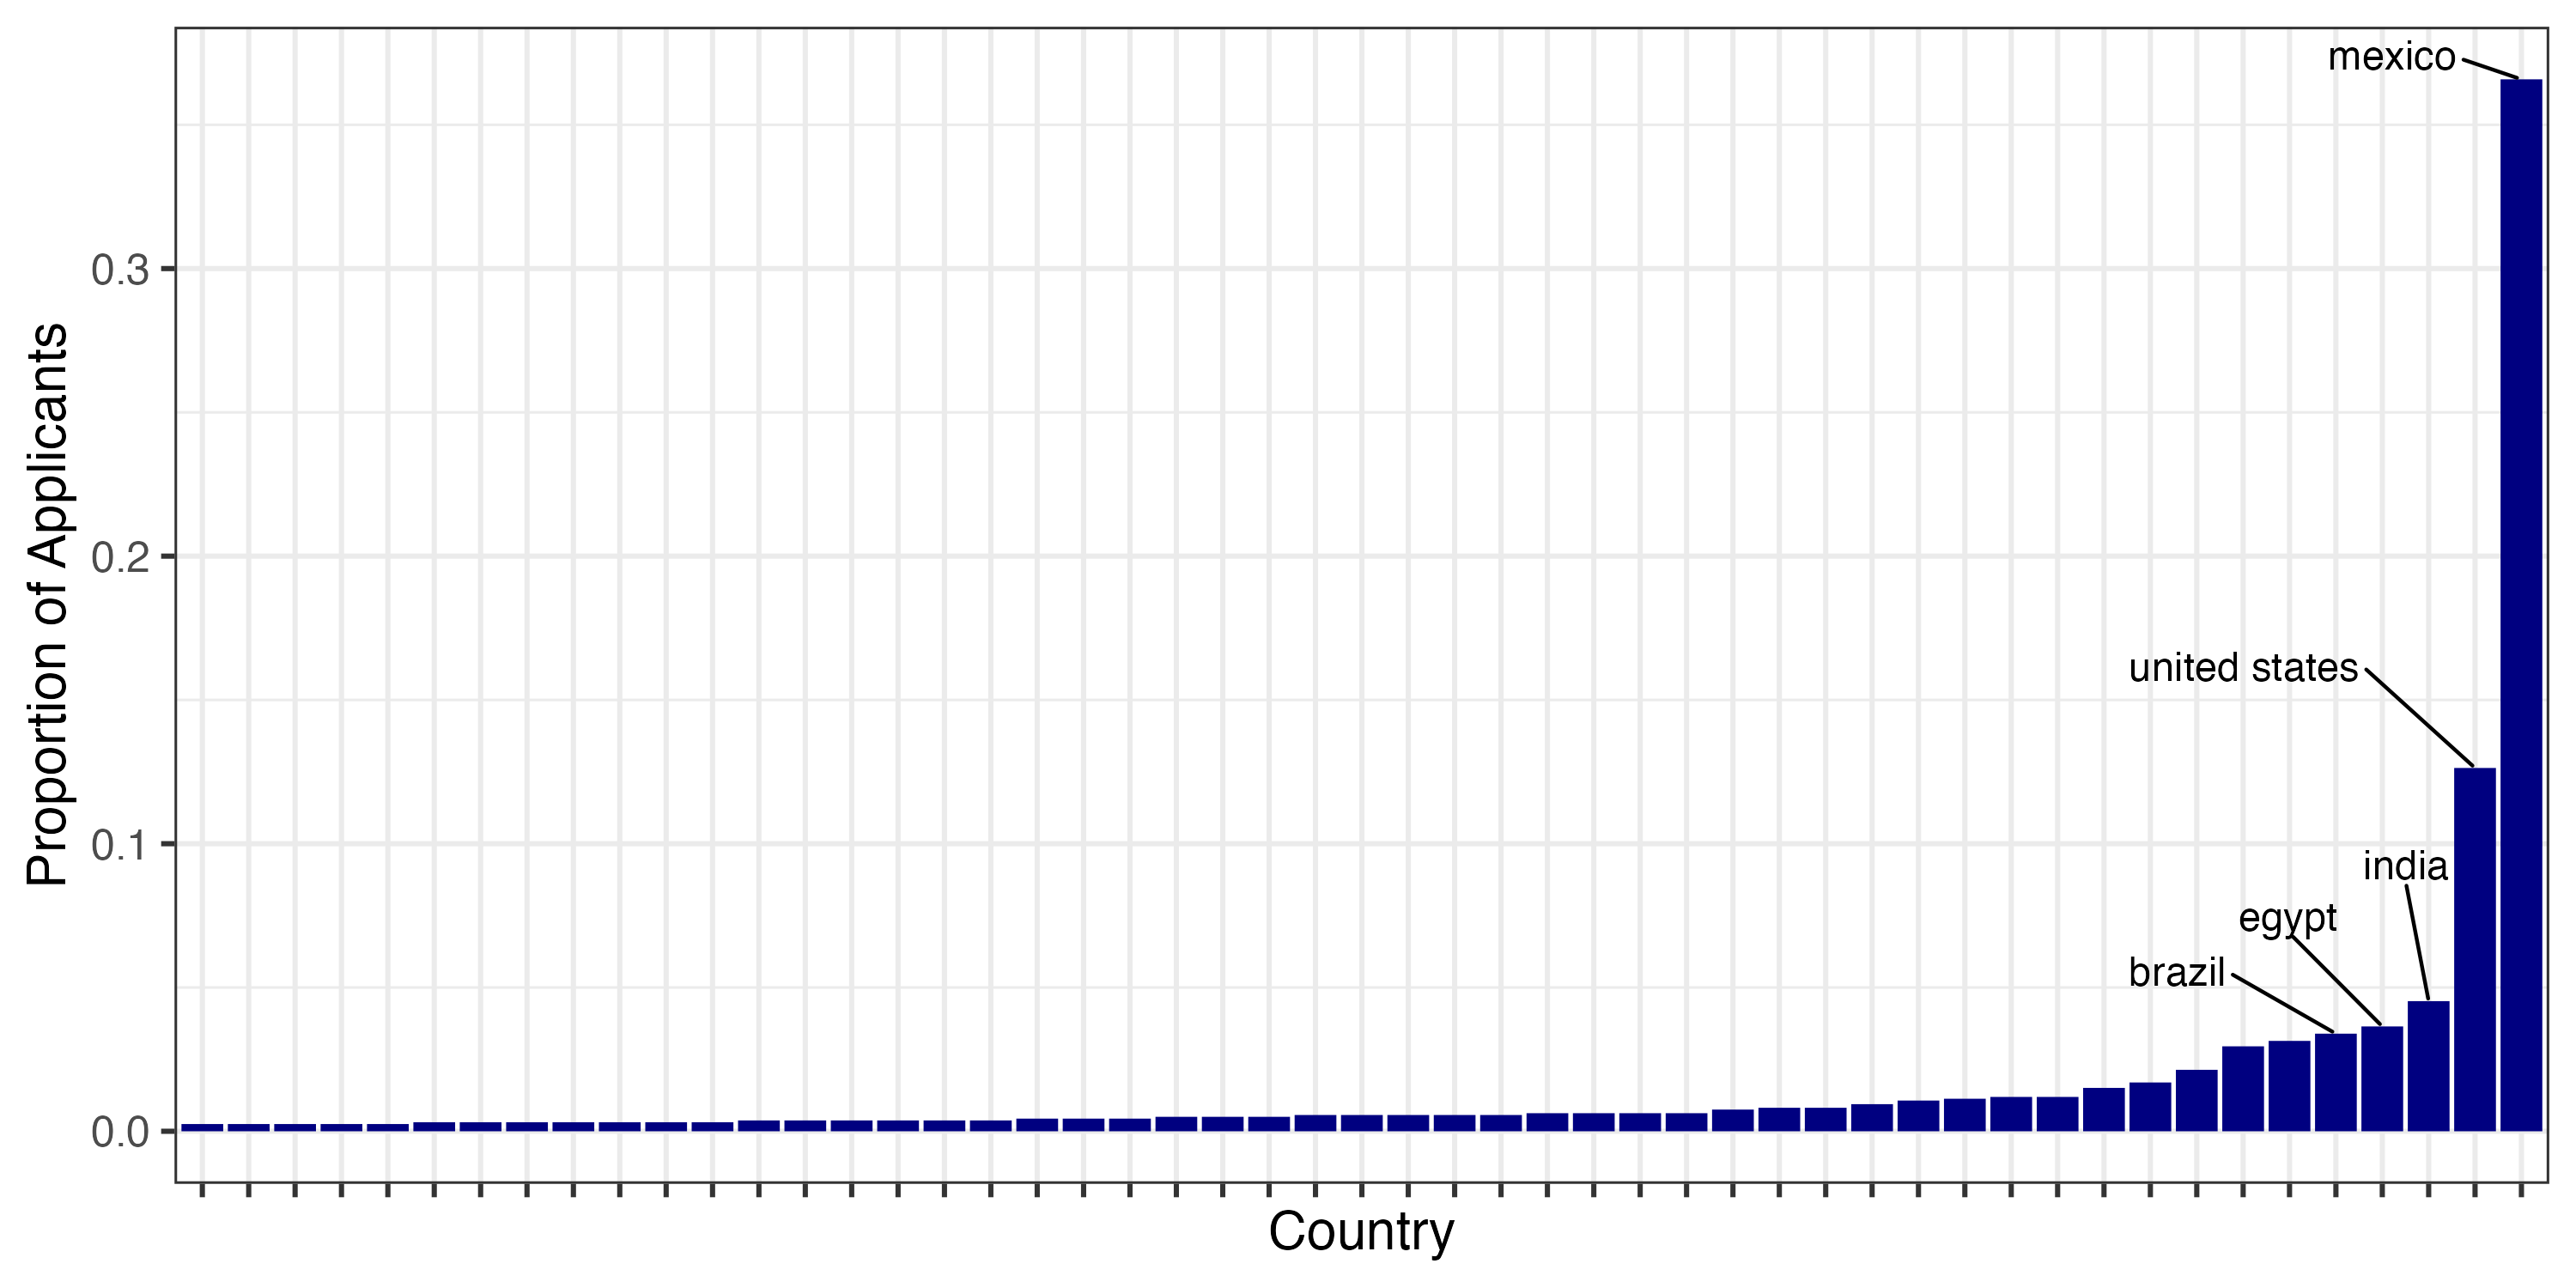
\includegraphics[width=1.3\textwidth,height=\textheight,keepaspectratio]{spf/candidate_countries_yr1.png} 
    % \end{figure}
    
    
    % \newpage
    % \begin{figure}[!htb]
    % \centering
    %     \caption{ This figure displays the SPFs we estimate for three finalist cohorts. The y-axis represents the diversity score while the x-axis represents average cohort performance (i.e. percentiles of mean project scores). The diversity target is held constant across cohorts, so differences in SPFs conditional on performance represent differences in the capacity to reach the same diversity target at a given level of performance.}\label{fig:diversity_across_cohorts}
    %   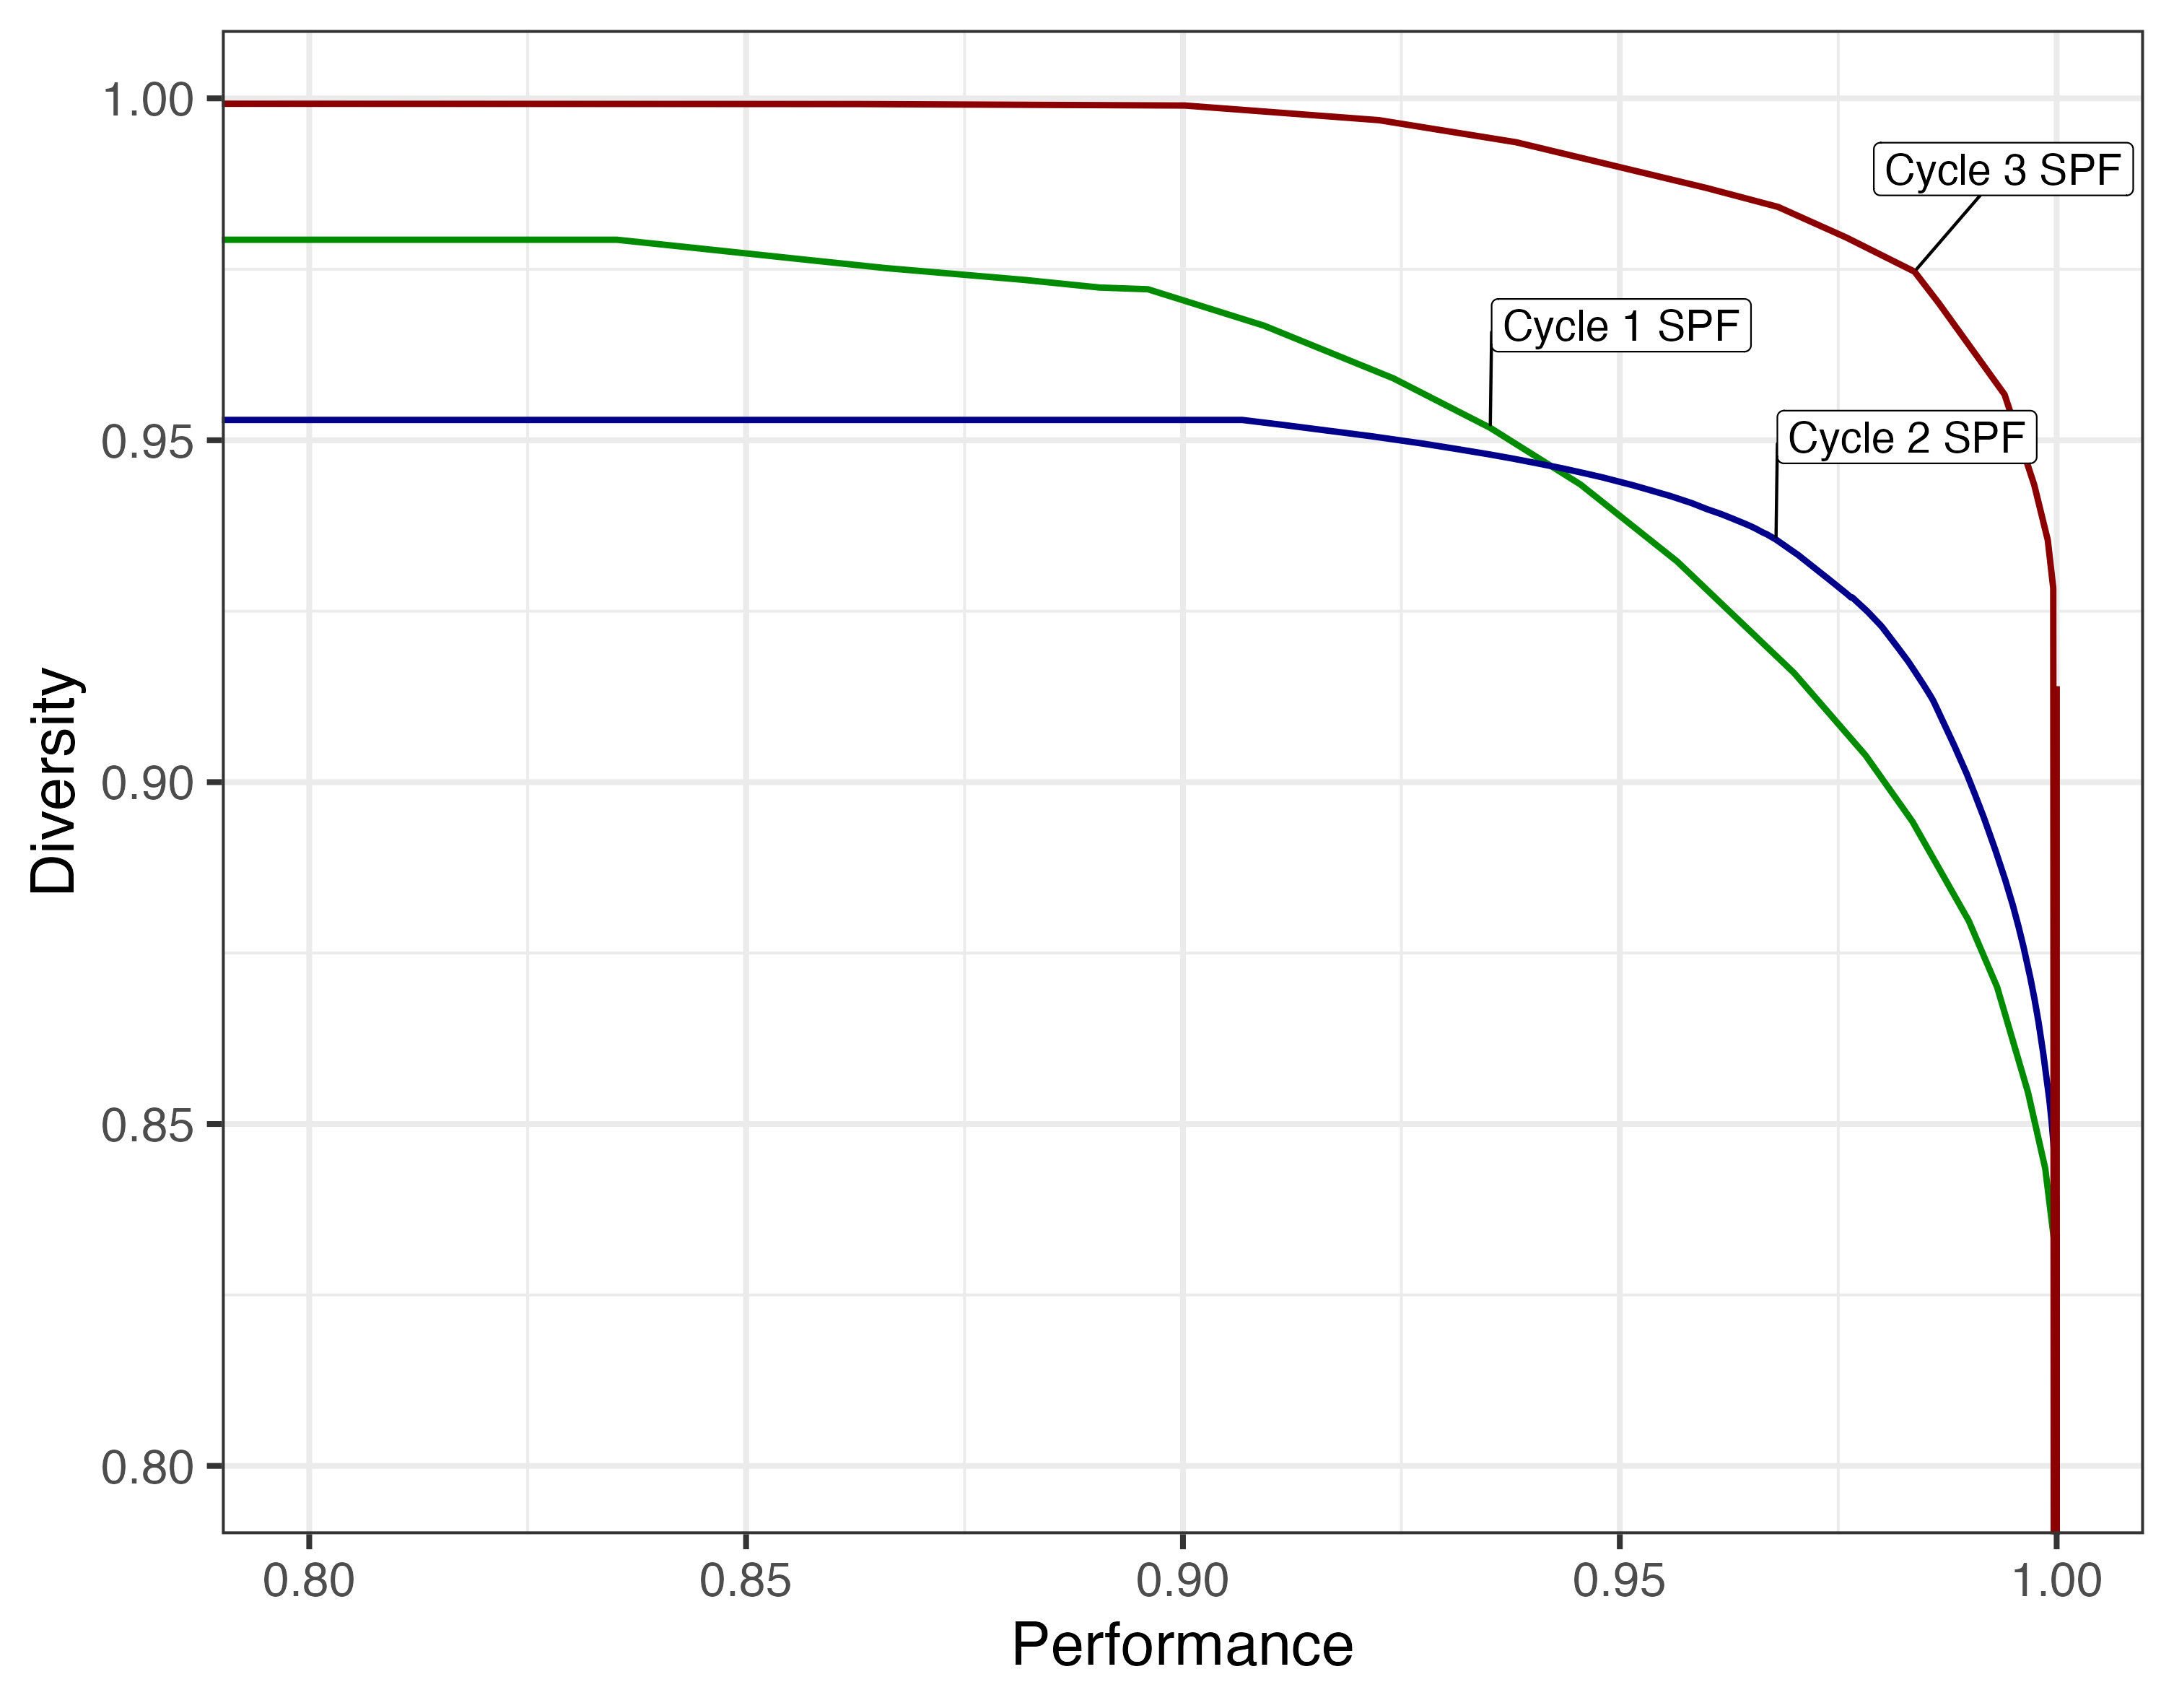
\includegraphics[width=\textwidth,height=\textheight,keepaspectratio]{spf/spf_cohort_comparisons.png} 
    % \end{figure}
    
    % \newpage
    % \newpage
    % \begin{figure}[!htb]
    %     \centering
    %     \caption{This figure shows example screens that expert reviewers saw when rating essays (Panel \ref{subfig:essay}) and project presentations (Panel \ref{subfig:project}). Both were rated on 15 point scales judging effectiveness and impressiveness of the project. Text of the example project essay and the face of the applicant have both been blurred to protect the identity of the applicants. }
    %     \begin{subfigure}[]{\textwidth}
    %         \centering
    %                 \caption{Project Essay Review Screen} \label{subfig:essay}
    %         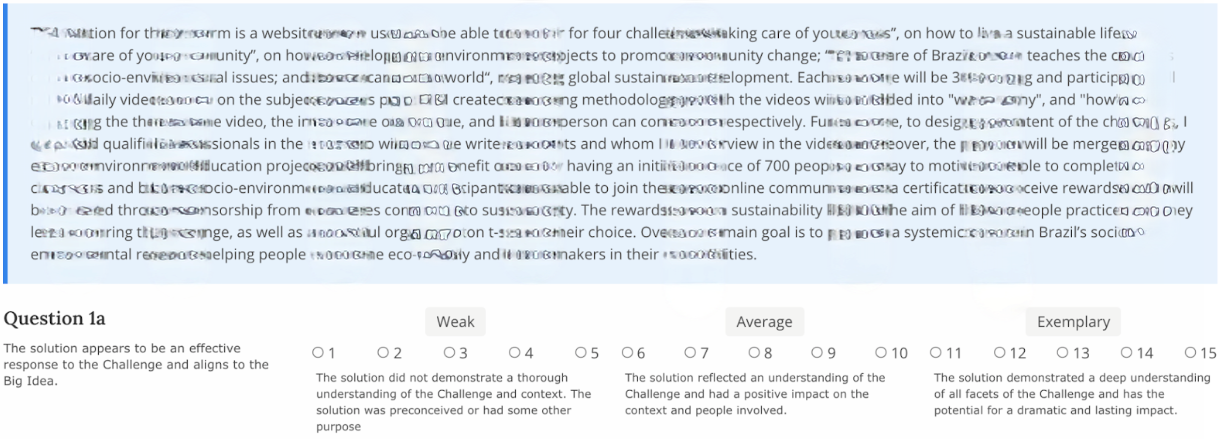
\includegraphics[width=\linewidth]{spf/essay_review_screen.png} 
    %     \end{subfigure}
        
    %     \hfill
    %     \vspace{1em}
    %     \begin{subfigure}[]{\textwidth}
    %         \centering
    %                 \caption{Final Project Review Screen} \label{subfig:project}
    %         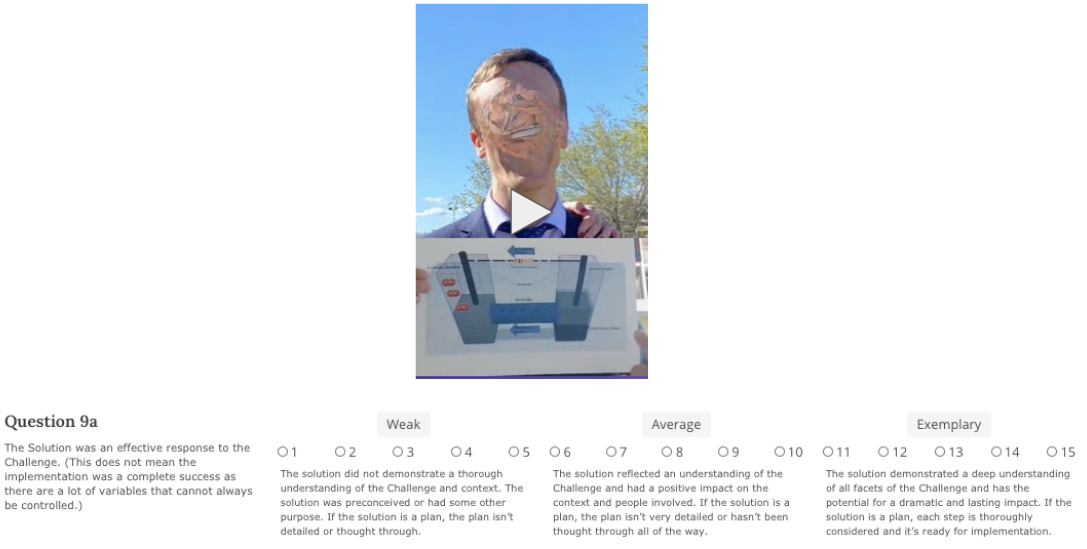
\includegraphics[width=\linewidth]{spf/project_review_screen.png} 
    %     \end{subfigure}
        
    % \end{figure}
    
    
    % \newpage
    
    % \null
    % \vfill
    % \begin{figure}[!htb]
    % \centering
    % \caption{This figure shows sample items for all three types of questions the programme used from International Cognitive Ability Resource (ICAR) assessment. All three item types are best described using language from the ICAR website: the Cube Rotation items "present participants with cube renderings and ask participants to identify which of the response choices is a possible rotation of the target stimuli", the Number Sequence items ask participants to " fill in one or two numbers that follow in the sequence", and the Matrix Reasoning items "contain stimuli that are... 3x3 arrays of geometric shapes with one of the nine shapes missing" (similar to those used in Raven's Progressive Matrices) and participants "are instructed to identify which of six geometric shapes presented as response choices will best complete the stimuli". Because the applicant pool was international, these specific item types were chosen because they rely minimally on knowledge of english. In the programme's implementation, each applicant saw 5 questions of each type.}\label{fig:icar_items}
    % 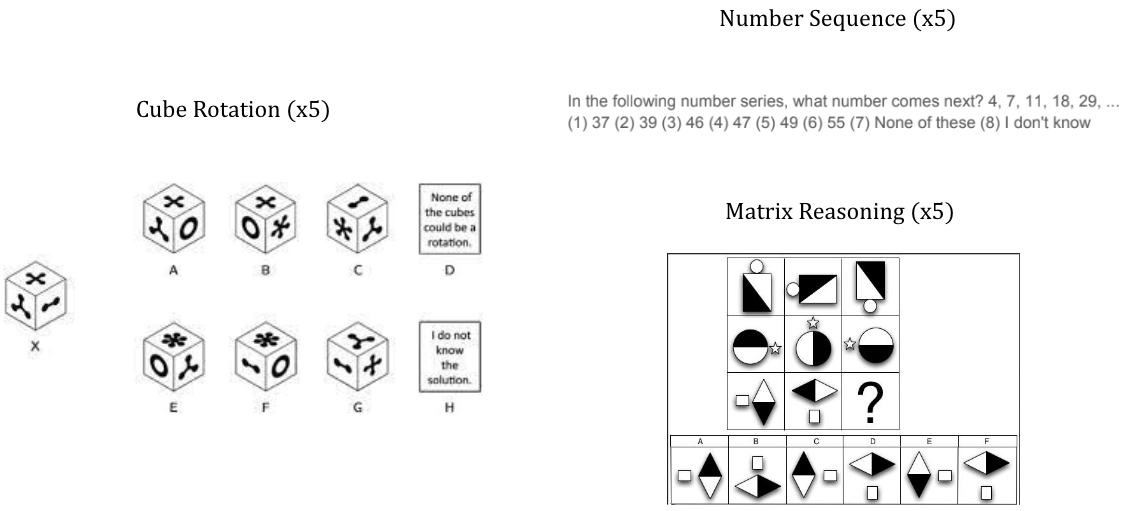
\includegraphics[width=1.3\textwidth,height=\textheight,keepaspectratio]{spf/icar_items.png} 
    % \end{figure}
    % \vfill
    
    
    % \newpage
    % \null
    % \vfill
    % \begin{figure}[!htb]
    % \centering
    %     \caption{The gamified skills test applied to applicants in cohort 3 is a game called Roomworld, and a sample level of the game is depicted above. In each level, applicants are challenged to move through the grid using the arrow keys to get the yellow icon to the gift. Shapes within the grid serve as different obstacles and mechanisms for navigating the level. How each obstacle and mechanism work are not explained to the player, as part of the test is about discovering \emph{how} they work. Multidimensional data from the game are collected and aggregated to give players a percentile score. The specific scoring alorithm was developed by researchers in the Human Information Processing Lab at Oxford university and has not been provided to us.}\label{fig:roomworld_instance}
    % 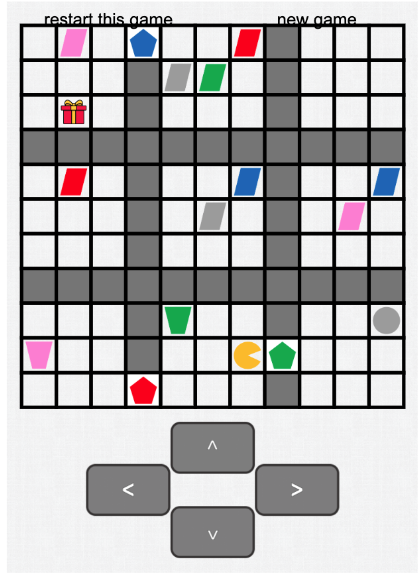
\includegraphics[width=.6\textwidth,height=\textheight,keepaspectratio]{spf/roomworld_instance.png} 
    % \end{figure}
    % \vfill
    
    % \newpage
    % \begin{figure}[!htb]
    % \centering
    %     \caption{This figure depicts various binscatter plots that reveal the association between college rank and expert-judged project performance. Data used for these plots come from two sources: (1) 121 respondents to a follow-up survey administered to cycle 1 and cycle 2 programme applicants and (2) 359 respondents to a survey administered to cohort cycle 2 finalists. In the former, school rank comes from the respondents' self-reported college at which they have matriculated. But, in the latter, school rank is based on the schools that respondents are most interested in attending (i.e. the college they aspire to attend). Panel A depicts the relationship between expert project reviews and school rank pooling together both samples. Panel B plots the relationship conditional on data source. Panel C is limited just to the follow-up survey. Panel D is limited just to the cohort cycle 2 finalists. In the top right of each panel is the coefficient of interest from regressions that correspond to each panel. *** significant at the 1\% level; ** significant at the 5\% level; * significant at the 10\% level} \label{fig:proj_robust_1}
    % 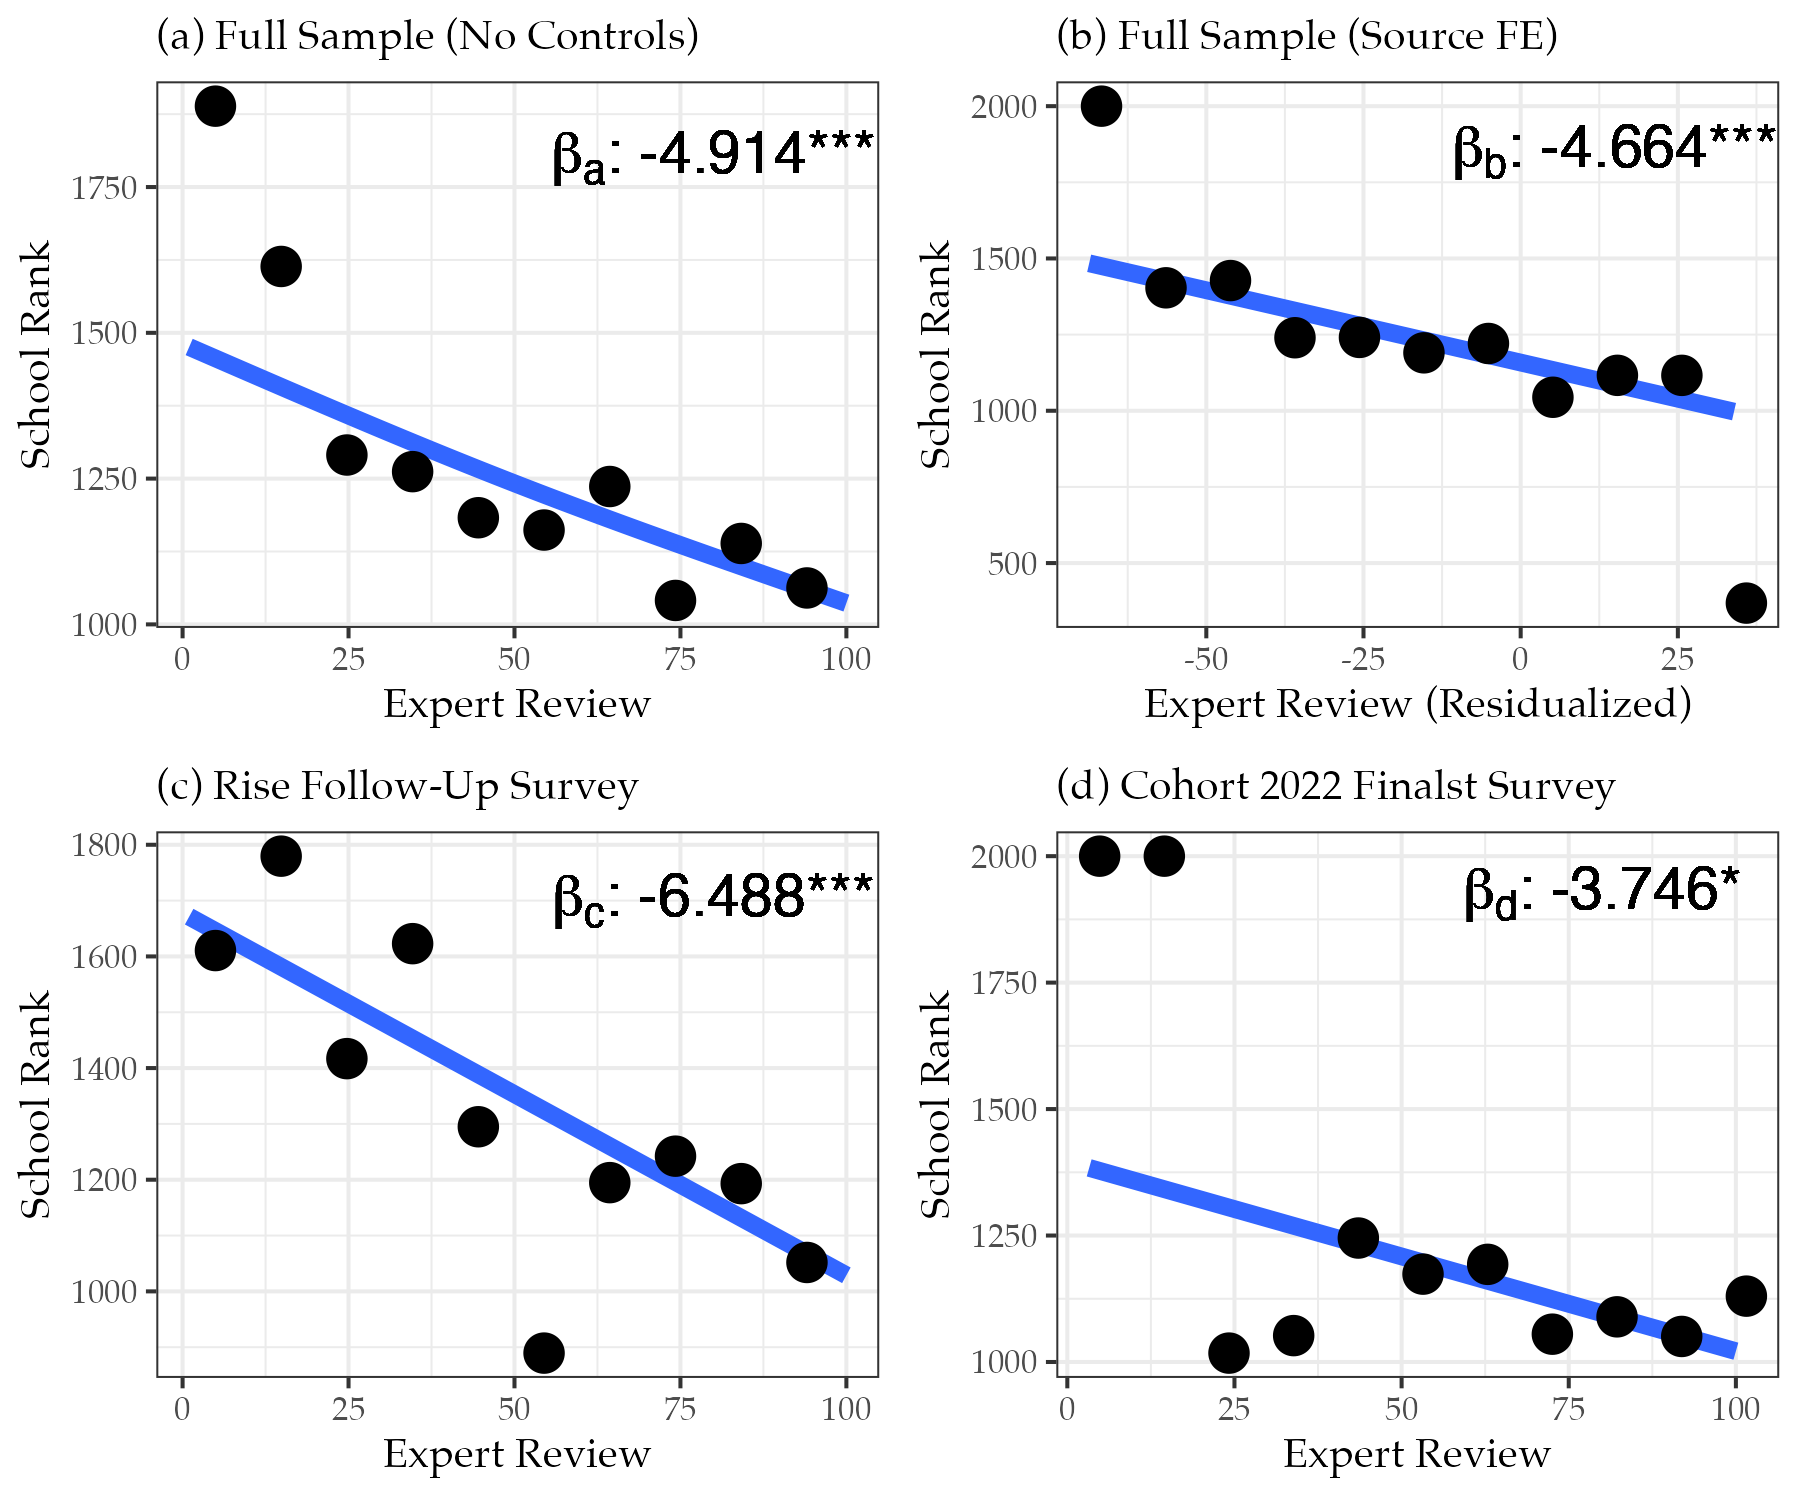
\includegraphics[width=.9\textwidth,height=\textheight,keepaspectratio]{spf/validation_raw.png} 
    % \end{figure}
    
    % \newpage
    % \begin{figure}[!htb]
    % \centering
    %     \caption{This figure depicts various binscatter plots that reveal the conditional association between college rank and expert-judged project performance. Data used for these plots come from two sources: (1) 121 respondents to a follow-up survey administered to cycle 1 and cycle 2 programme applicants and (2) 359 respondents to a survey administered to cycle 2 finalists. In the former, school rank comes from the respondents' self-reported college at which they have matriculated. But, in the latter, school rank is based on the schools that respondents are most interested in attending (i.e. the college they aspire to attend). Each association depicted is conditional on "SES Controls", which consist of fixed effects for gender, parental education, living in a poor country, and being in a poor household. Panel A depicts the association between school rank and residuals from a regression of expert project reviews on SES Controls in a sample the pools responses from both data sources. Panel B plots the same association, adding a data source fixed effect. Panel C limits just to the follow-up survey. Panel D is limits just to the cohort cycle 2 finalists. In the top right of each panel is the coefficient of interest from corresponding regressions. *** significant at the 1\% level; ** significant at the 5\% level; * significant at the 10\% level} \label{fig:proj_robust_2}
    % 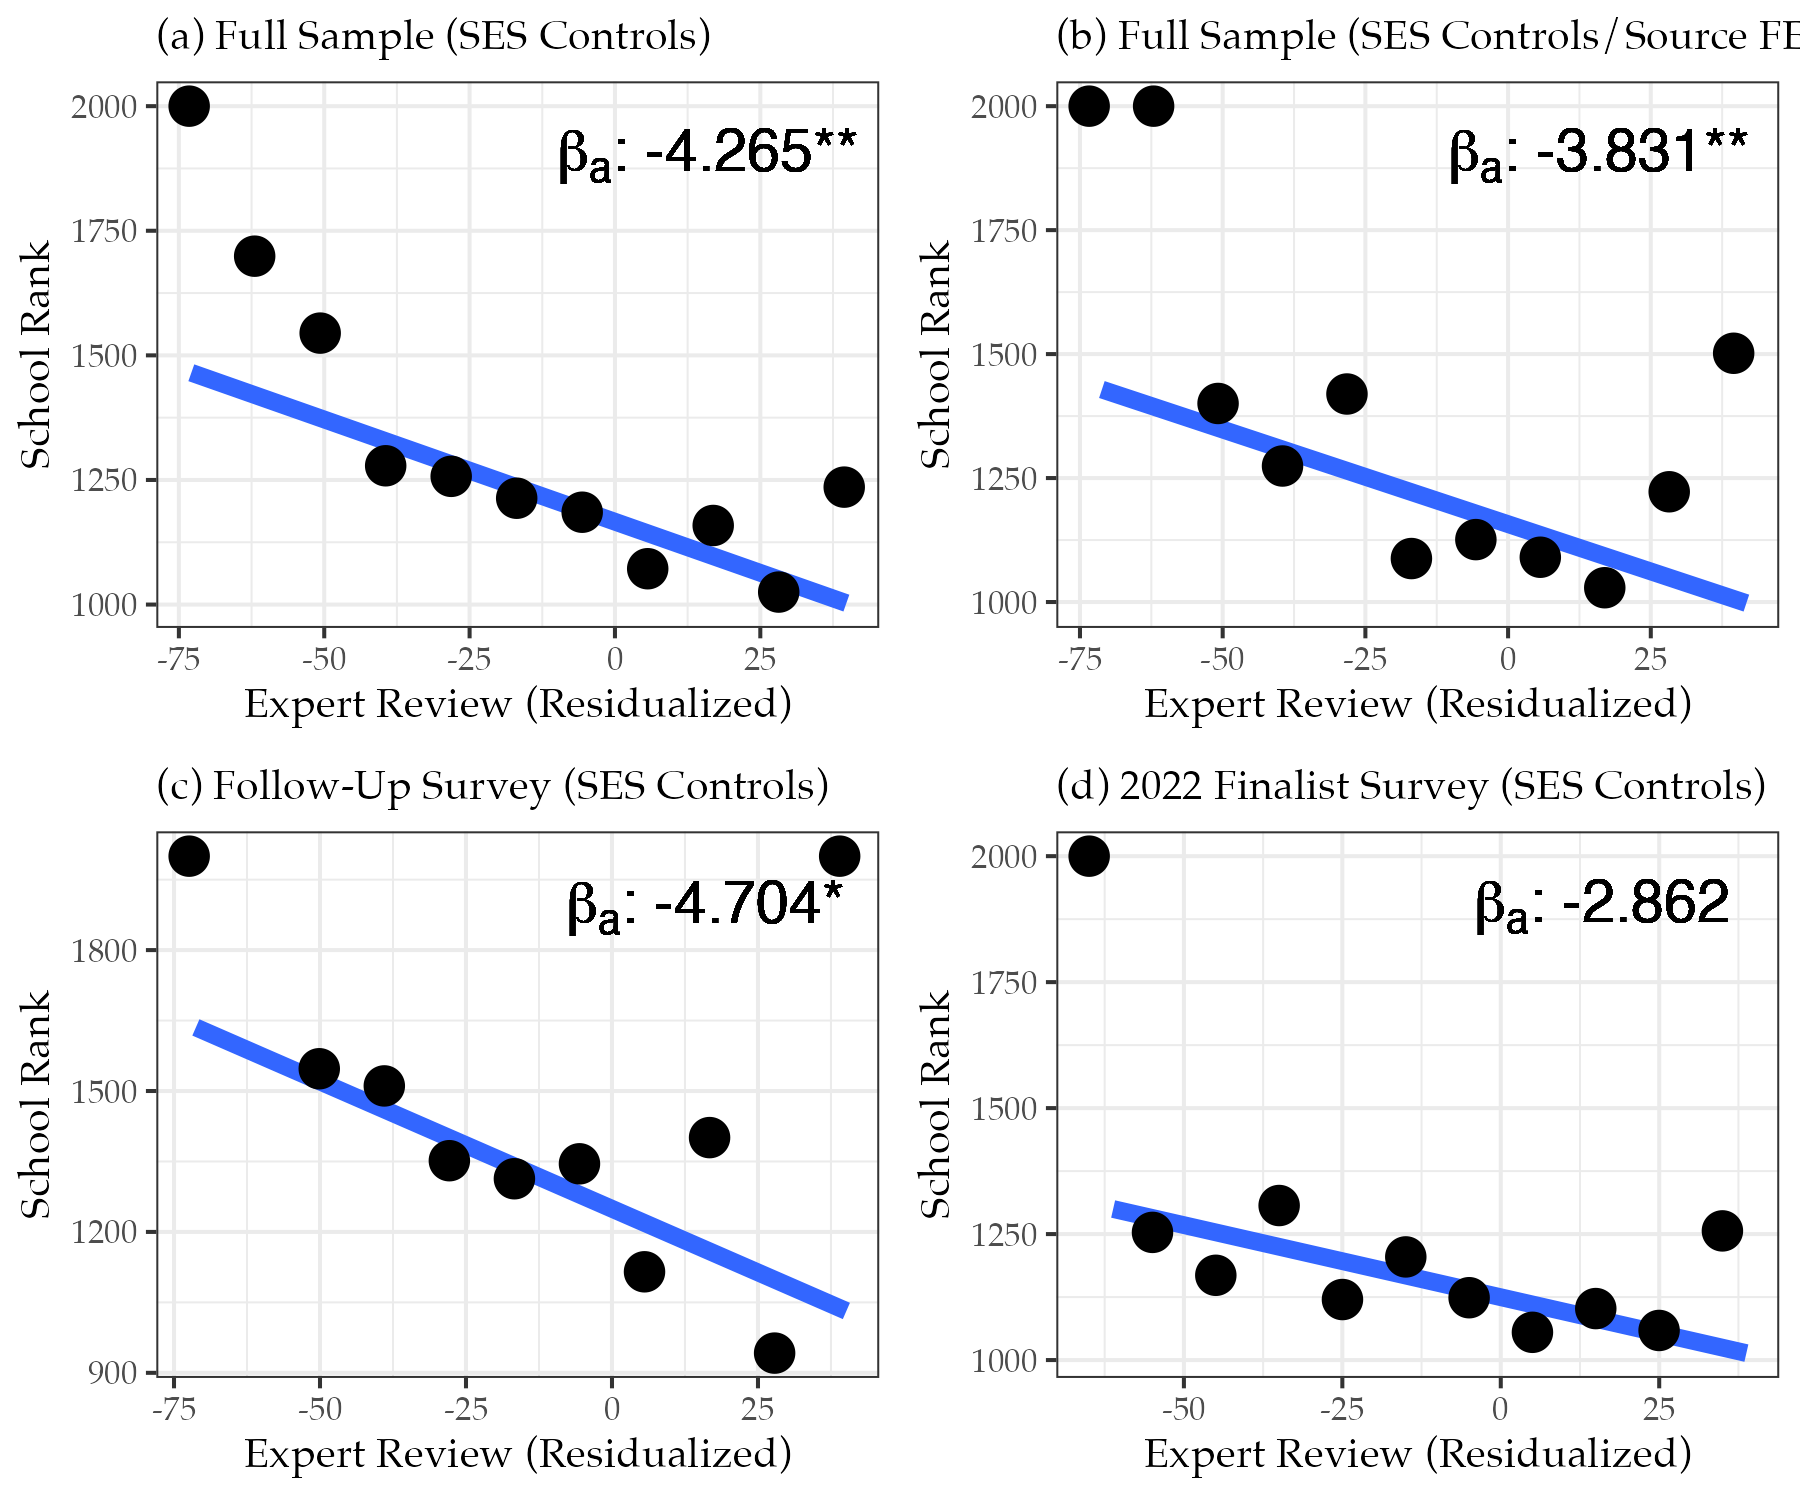
\includegraphics[width=.9\textwidth,height=\textheight,keepaspectratio]{spf/validation_w_controls.png} 
    % \end{figure}
    
    % \newpage
    % \begin{figure}[!htb]
    %     \centering
    %     \caption{Each panel in this figure depicts a binscatter intended to visualize the correlation between two potential screening scores (traditional and peer scores) and expert project performance scores. Panel \ref{subfig:trad_perf} depicts the relationship between the traditional score and project performance. Panel \ref{subfig:peer_perf} depicts the relationship between the peer score and project performance. Panel \ref{subfig:peer_trad} depicts the relationship between the peer score and the traditional score. }\label{fig:peer_ditr}
    %     \begin{subfigure}[t]{.45\textwidth}
    %         \centering
    %                 \caption{Traditional vs. Project Performance} \label{subfig:trad_perf}
    %         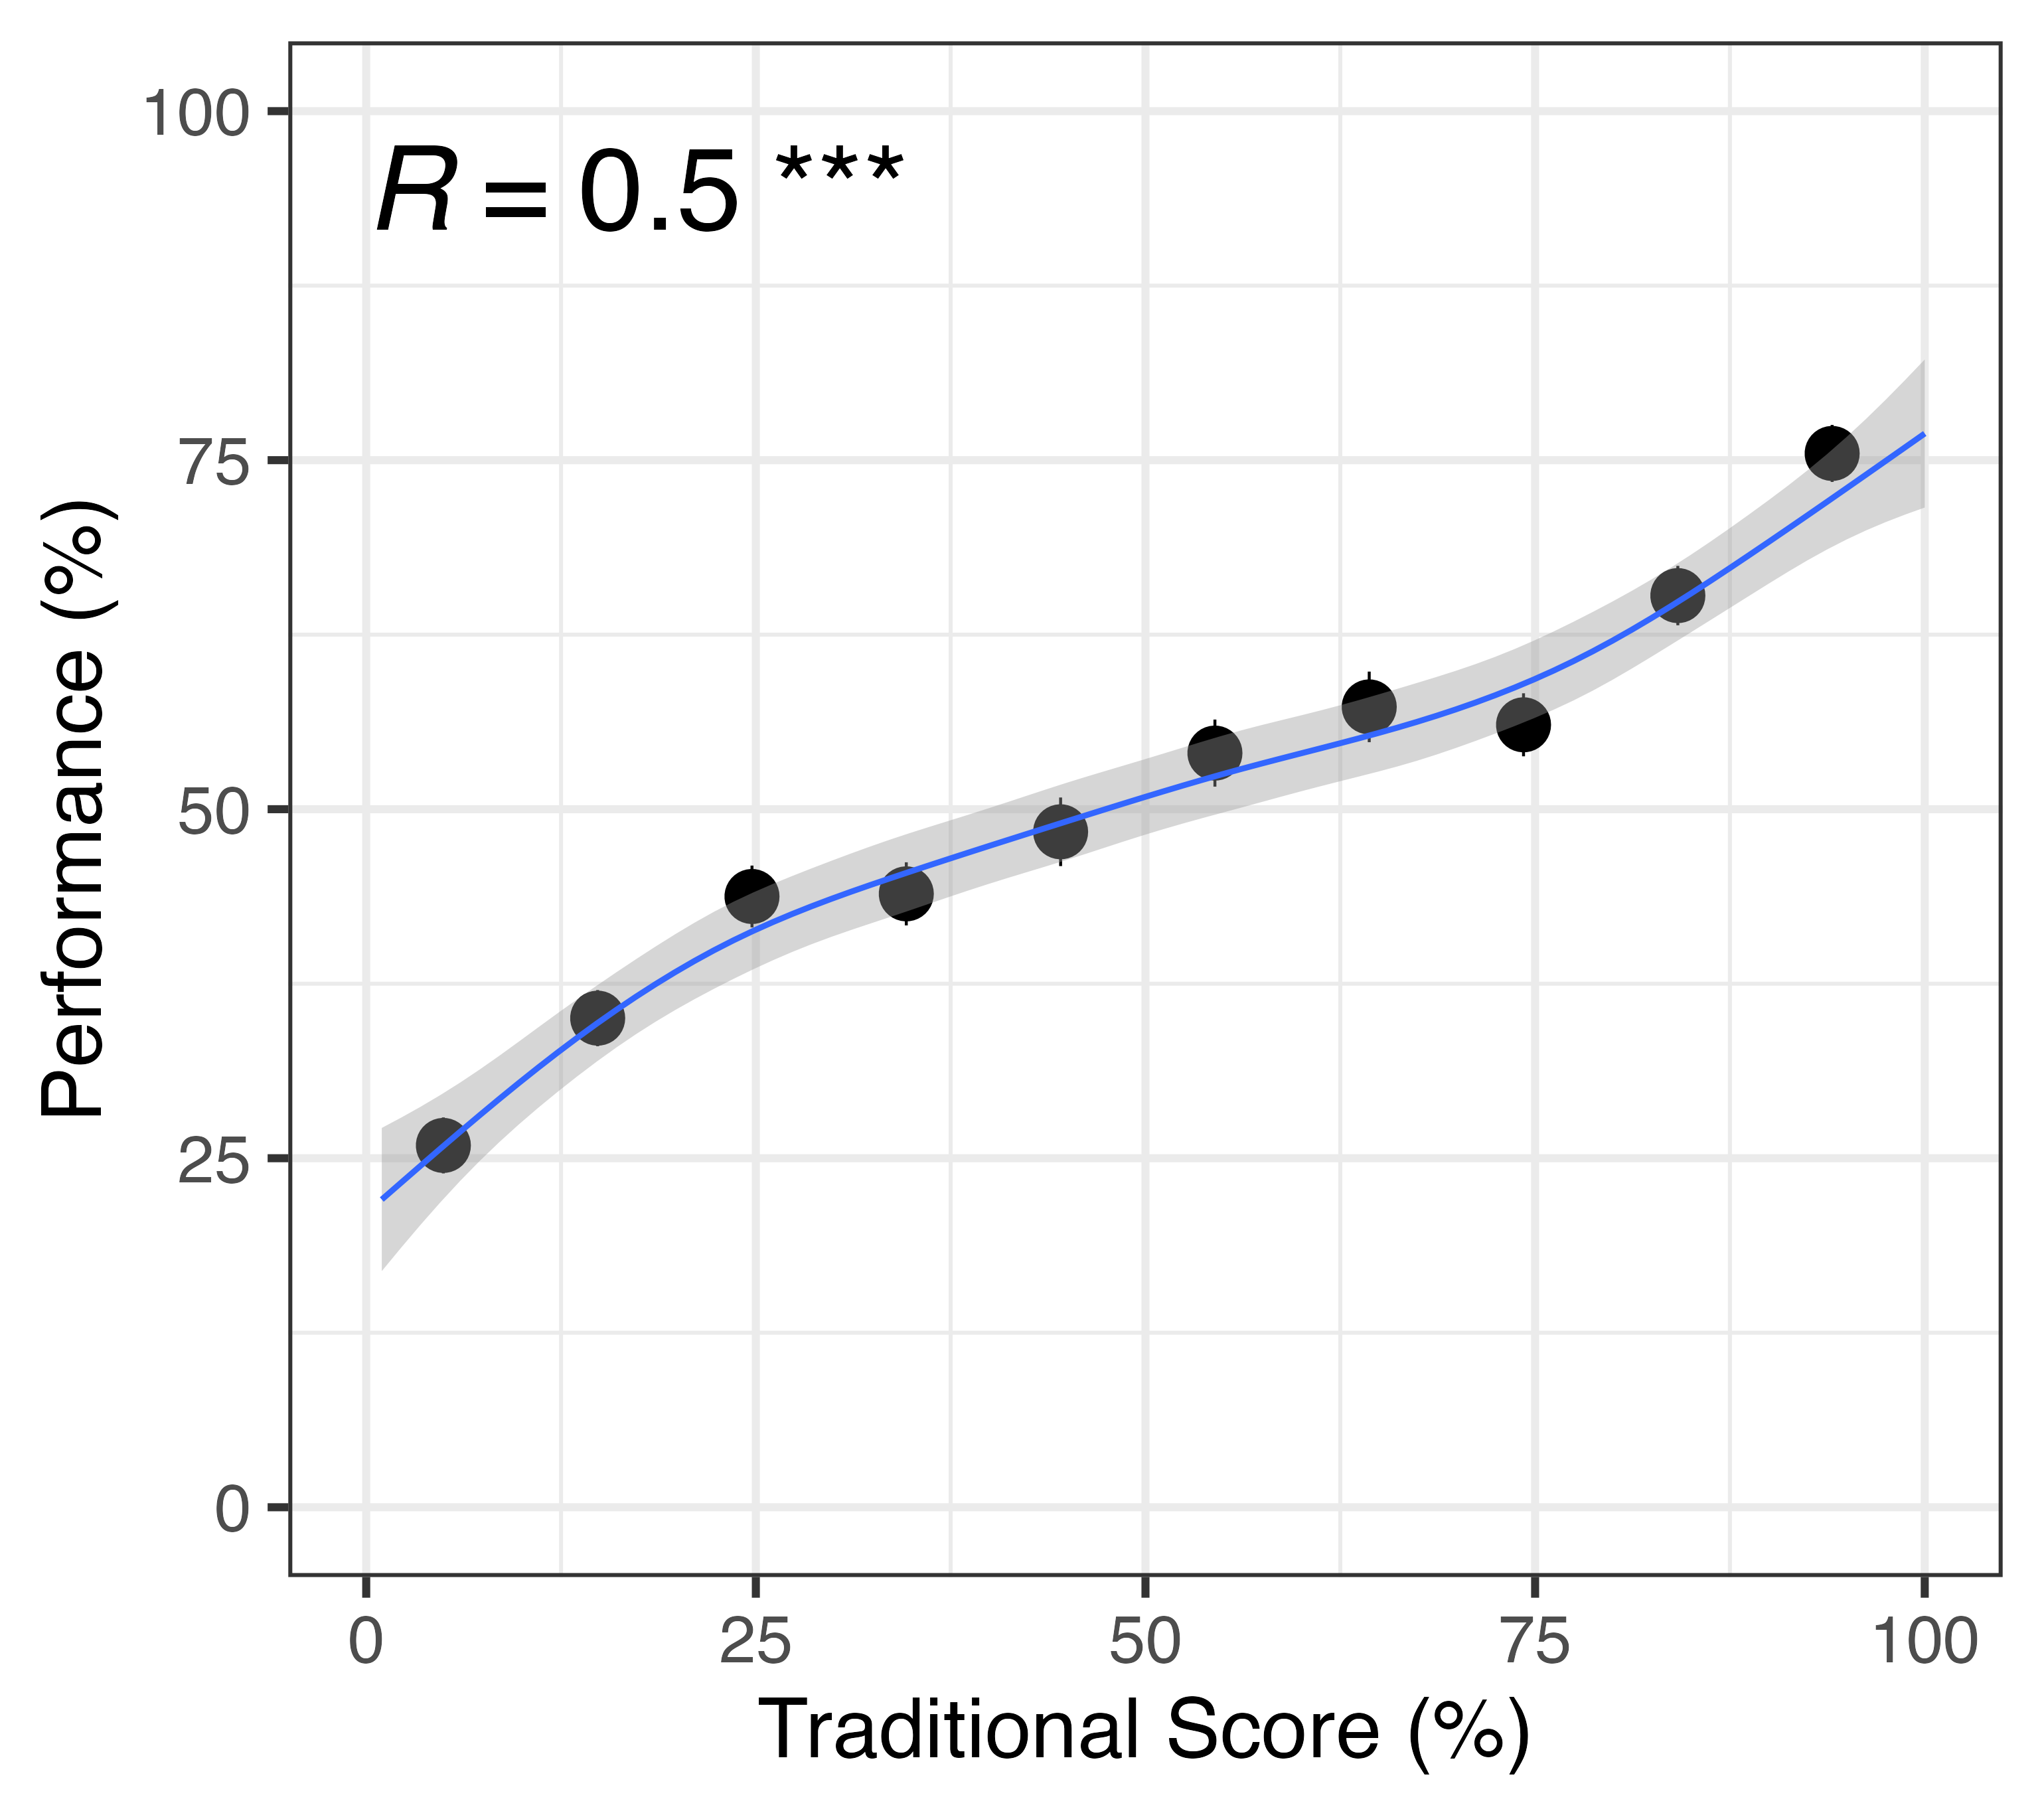
\includegraphics[width=\linewidth]{spf/traditional_performance_cor.png} 
    %     \end{subfigure}
    %     \hfill
    %     \vspace{1em}
    %     \begin{subfigure}[t]{.45\textwidth}
    %         \centering
    %                 \caption{Peer vs. Project Performance} \label{subfig:peer_perf}
    %         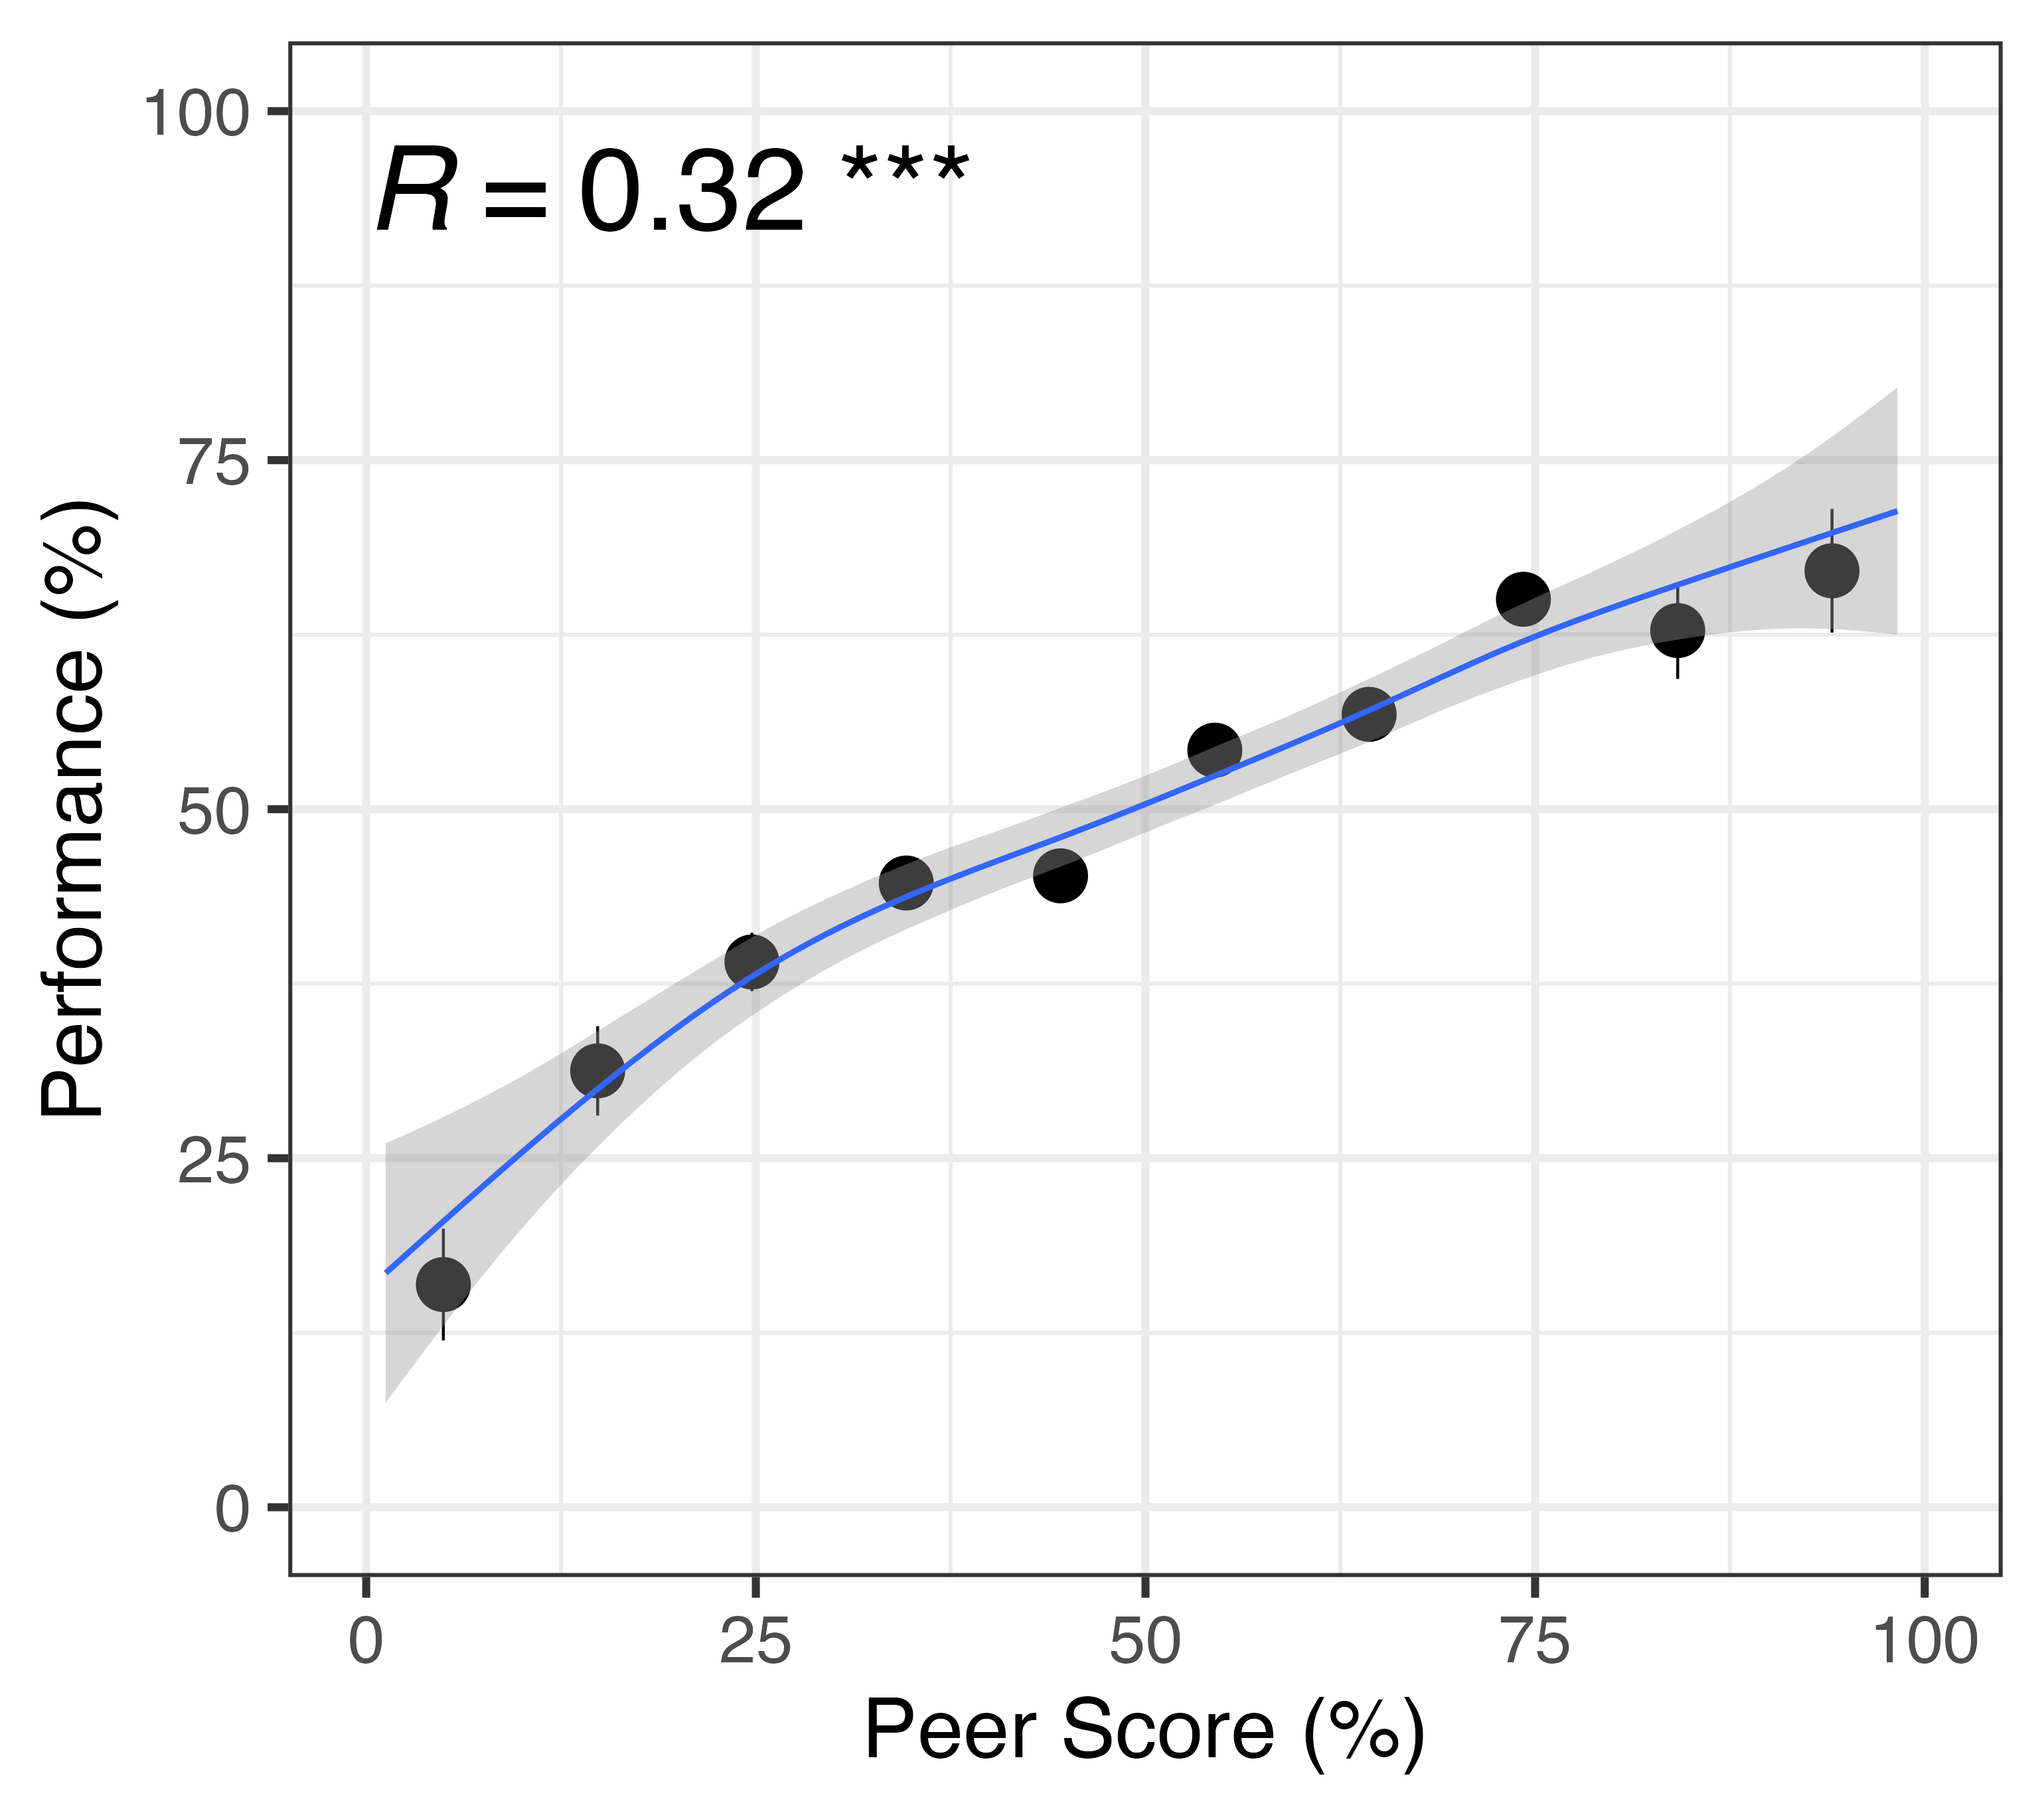
\includegraphics[width=\linewidth]{spf/peer_performance_cor.png} 
    %     \end{subfigure}
    %     \hfill
    %     \vspace{1em}
    %     \begin{subfigure}[t]{.45\textwidth}
    %         \centering
    %                \caption{Peer vs. Traditional} \label{subfig:peer_trad}
    %         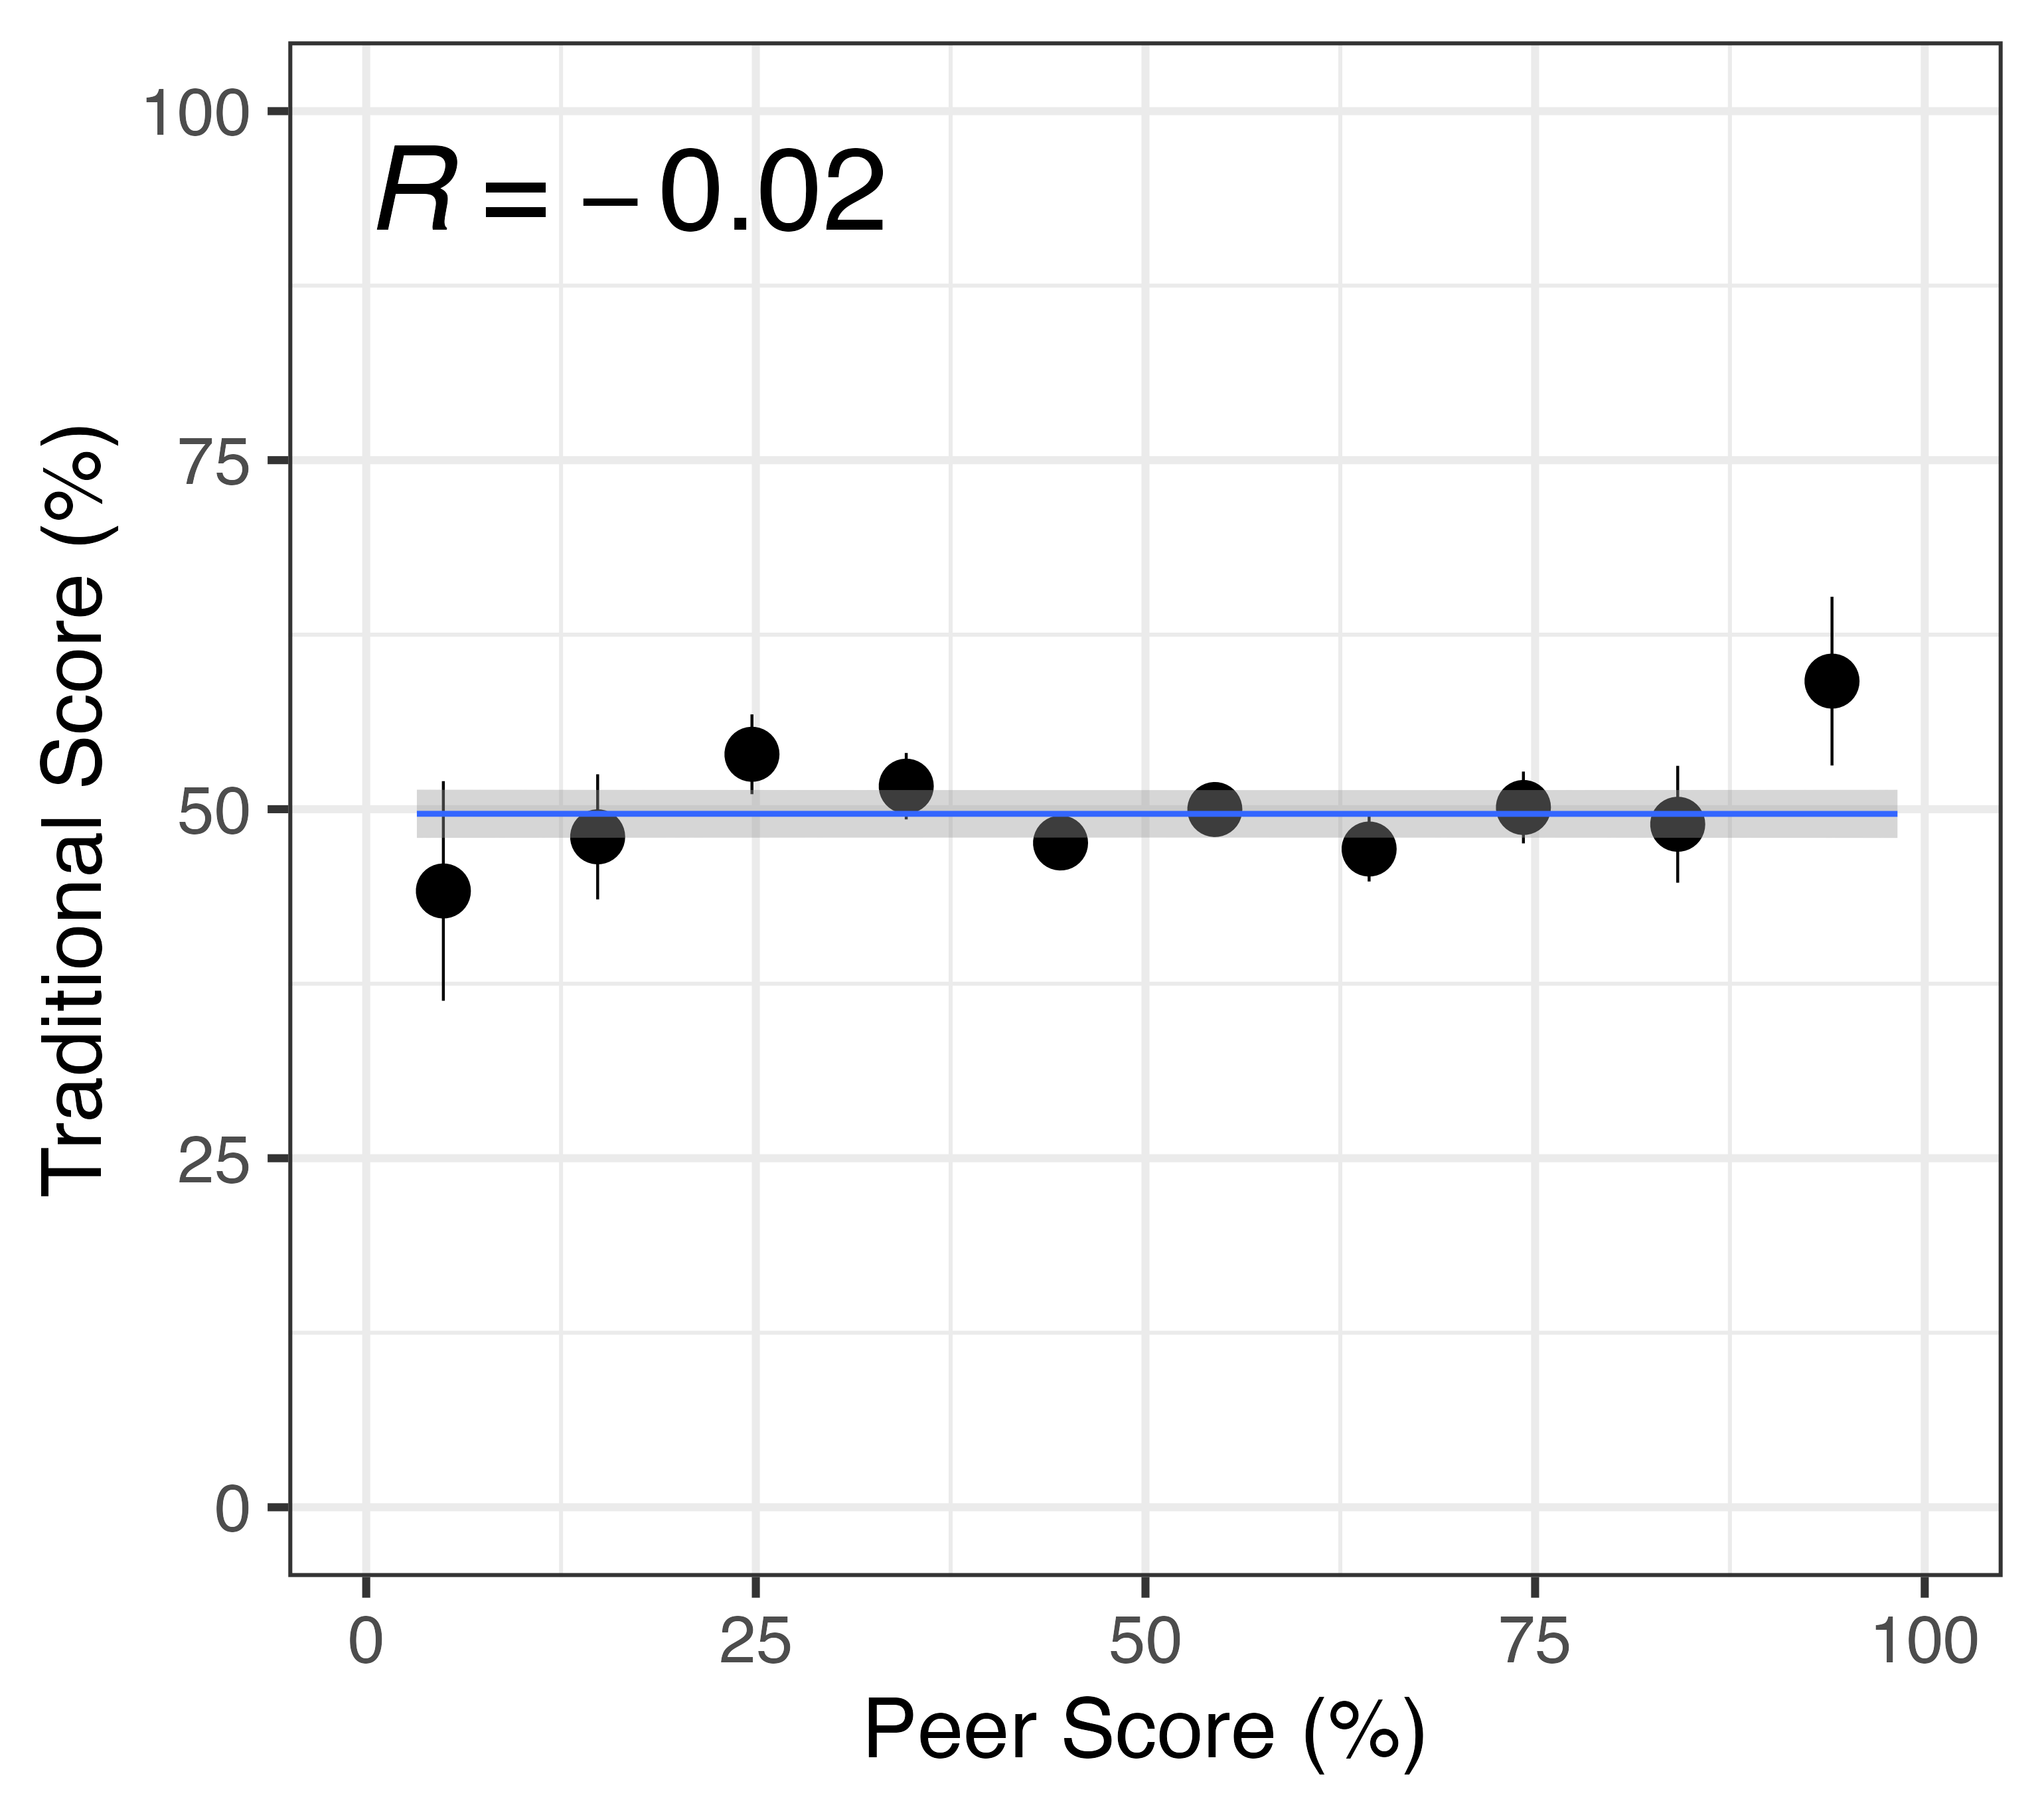
\includegraphics[width=\linewidth]{spf/peer_traditional_cor.png} 
    %     \end{subfigure}
    %         \hfill
    %     \vspace{1em}
    %      \begin{subfigure}[t]{.45\textwidth}
    %         \centering
    %                \caption{Peer vs. Project - Traditional} \label{subfig:peer_surp}
    %         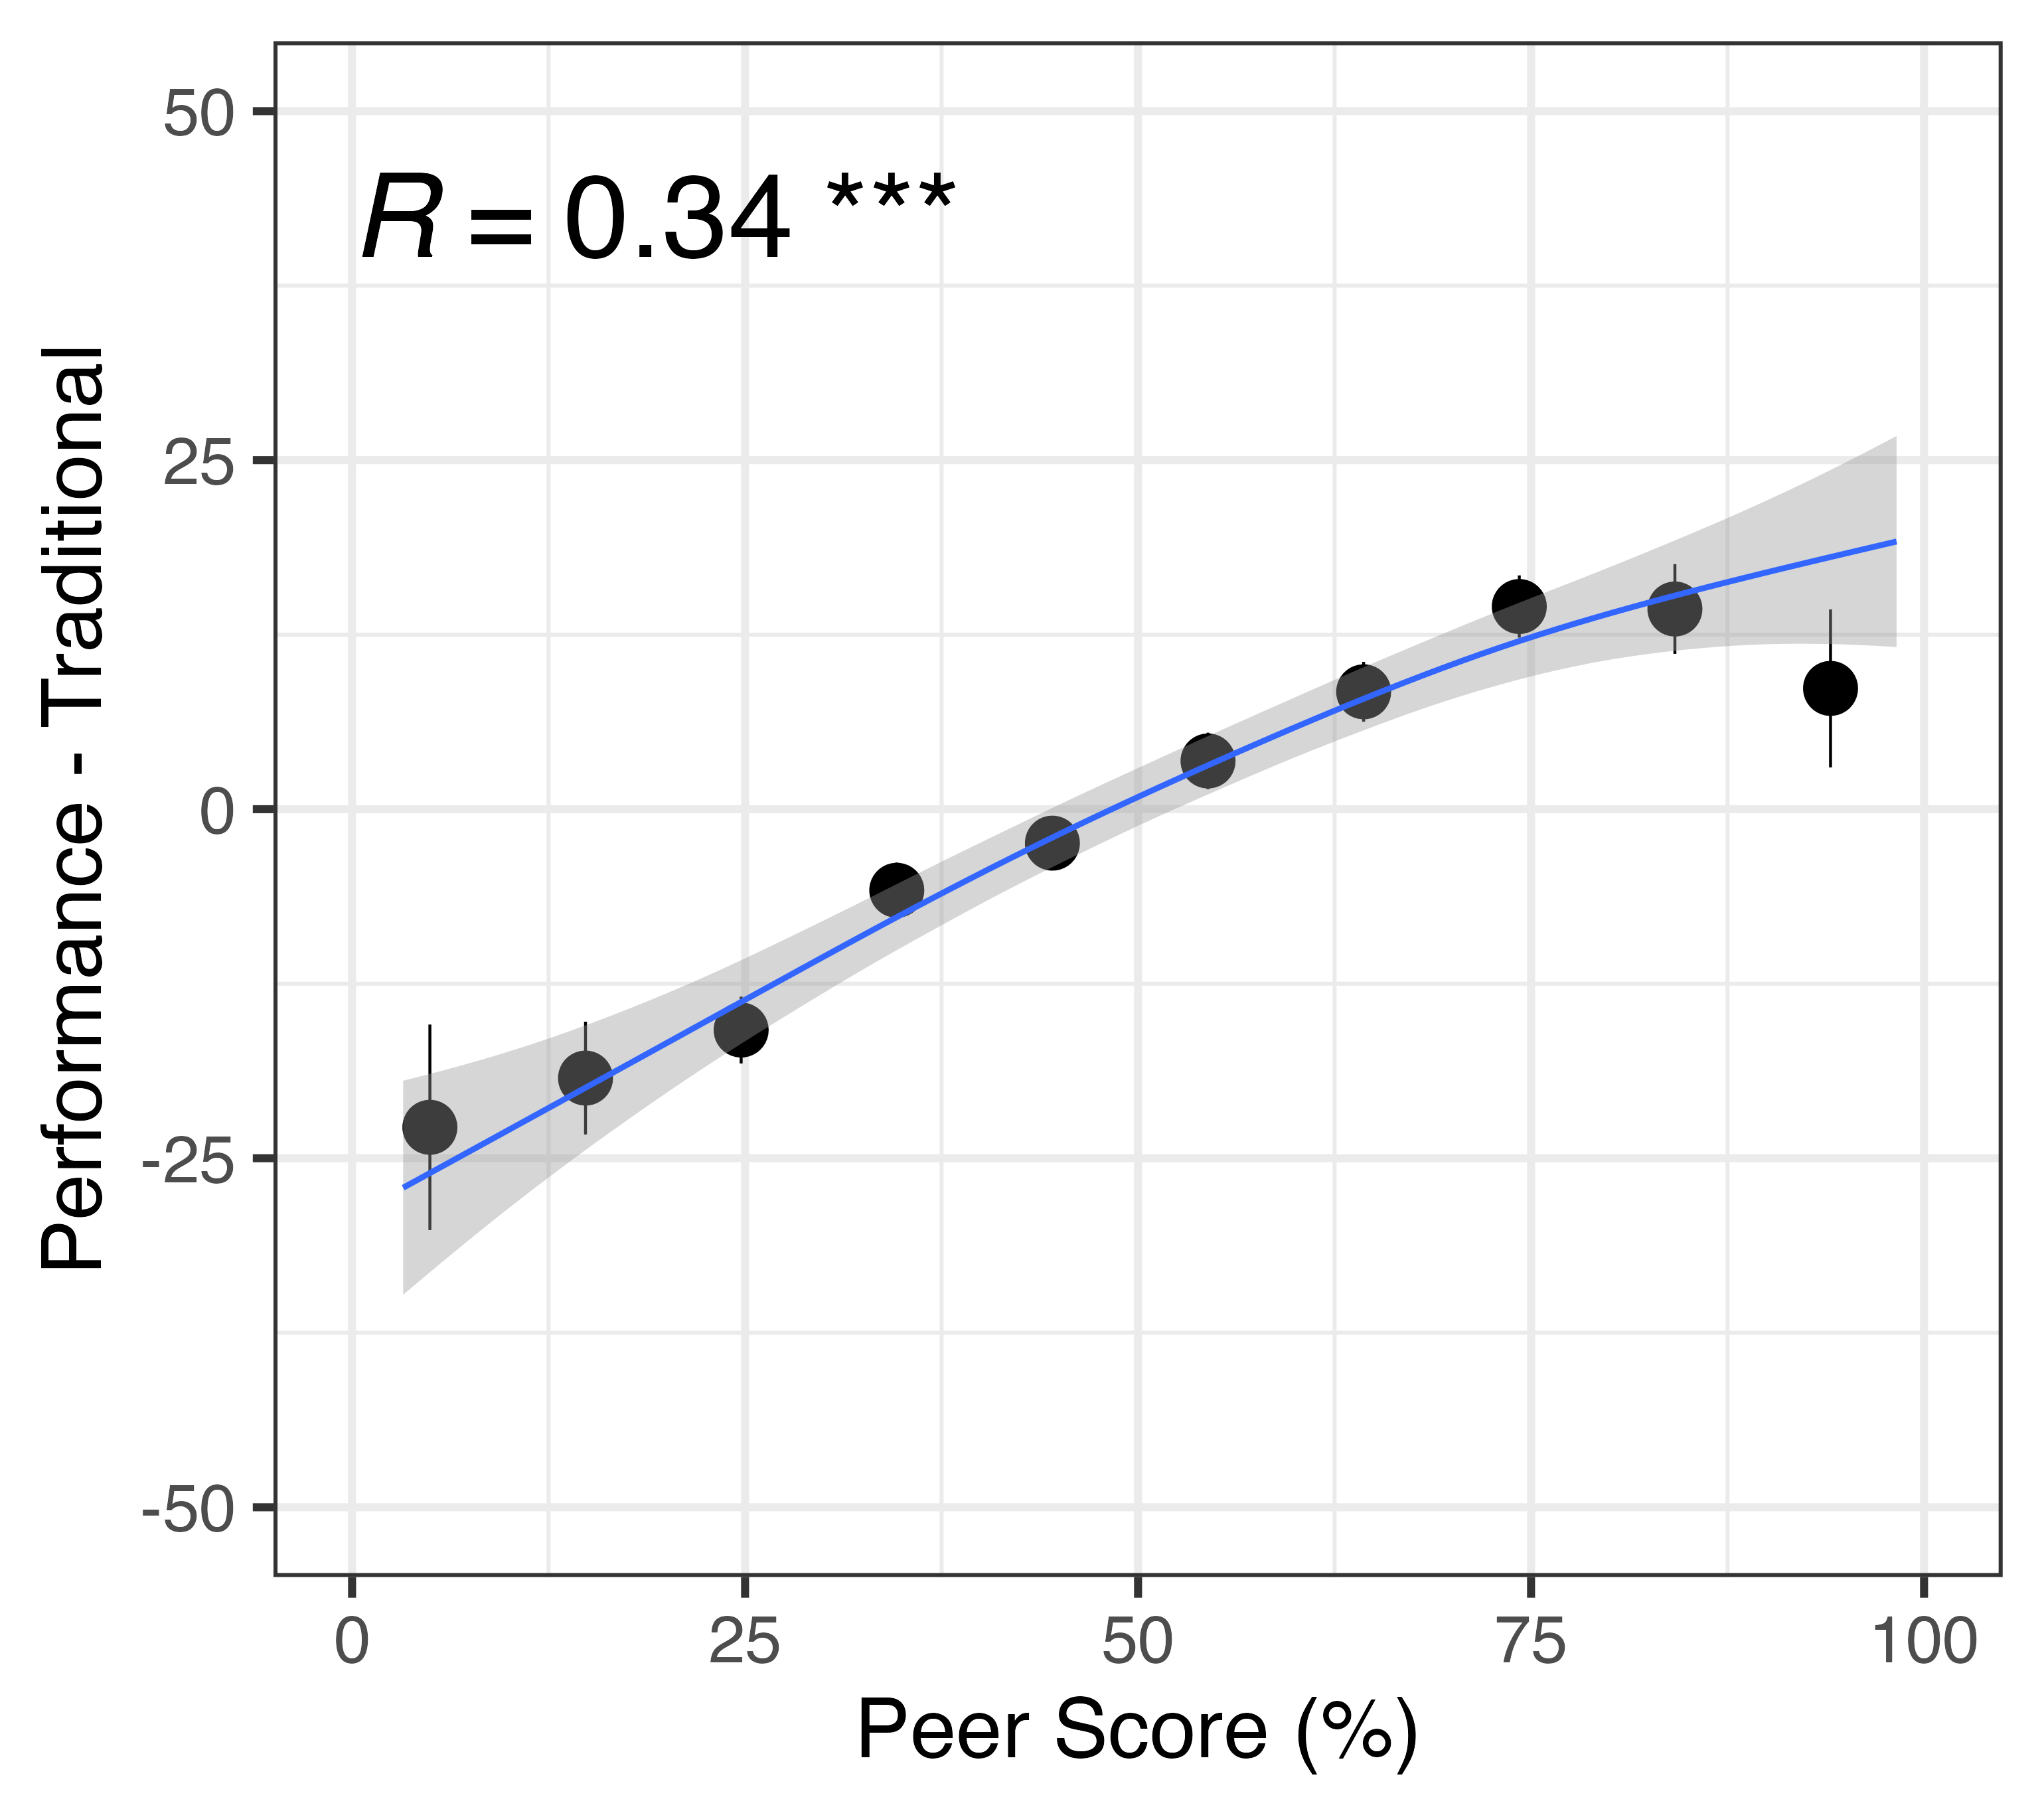
\includegraphics[width=\linewidth]{spf/peer_surprise_cor.png} 
    %     \end{subfigure}
    %             \hfill
    %     \vspace{1em}
    % \end{figure}
    
    % \newpage
    % \begin{figure}[!htb]
    % \centering
    %     \caption{This figure plots the percentile of average expert-judged project quality (i.e. performance) by deciles of cognitive, peer, and traditional scores for all three cohorts. The cognitive score is the percentile of the candidate's IQ, the peer score is the percentile of the average peer assessment of each applicant video, and the traditional score is the average percentile of a candidate's IQ and project essay rating.} 
    %     \label{fig:alt_talent_dist_full}
    %   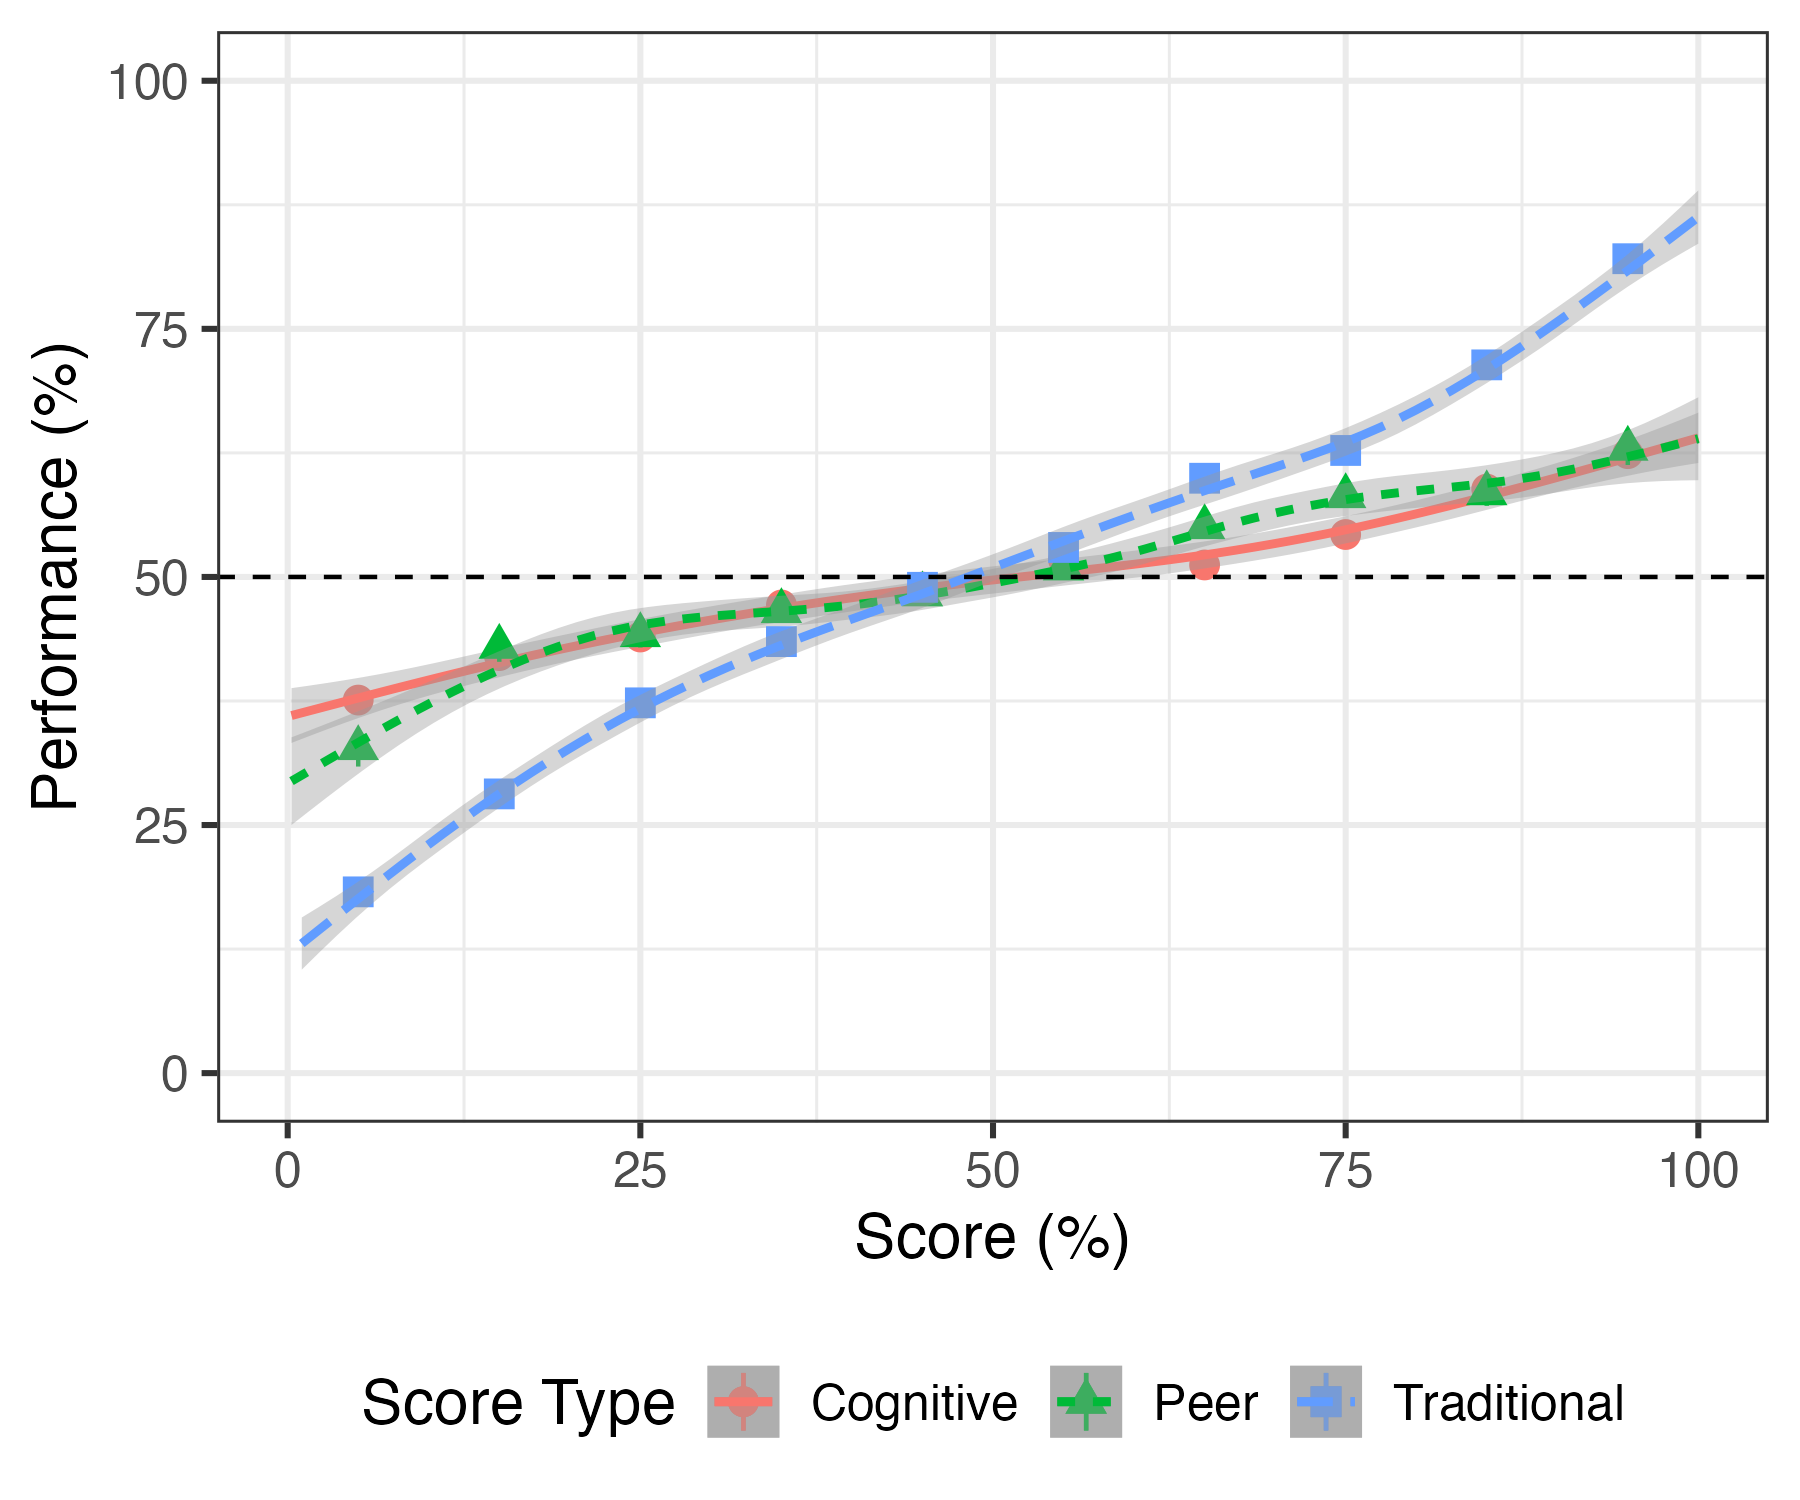
\includegraphics[width=\textwidth,height=\textheight,keepaspectratio]{spf/pq_by_scores.png} 
    % \end{figure}
    
    % \newpage
    % \begin{figure}[!htb]
    % \centering
    %     \caption{This figure plots the average of various measures of applicant socioeconomic (dis)advantage by deciles of cognitive, peer, and traditional scores for all three cohorts. The measures of (dis)advantage from Panel A to D in order are predicted mean parent income (yearly), years of education of most educated parent, whether or not the applicant lives in a globally poor household (mean parent income less than \$1,000 a year), and whether or not the applicant lives in a poor country (less than \$12,000 GDP per capita). The cognitive score is the percentile of the candidate's IQ, the peer score is the percentile of the average peer assessment of each applicant video, and the traditional score is the average percentile of a candidate's IQ and project essay rating. }
    %     \label{fig:disadvantage_corr_full}
    %   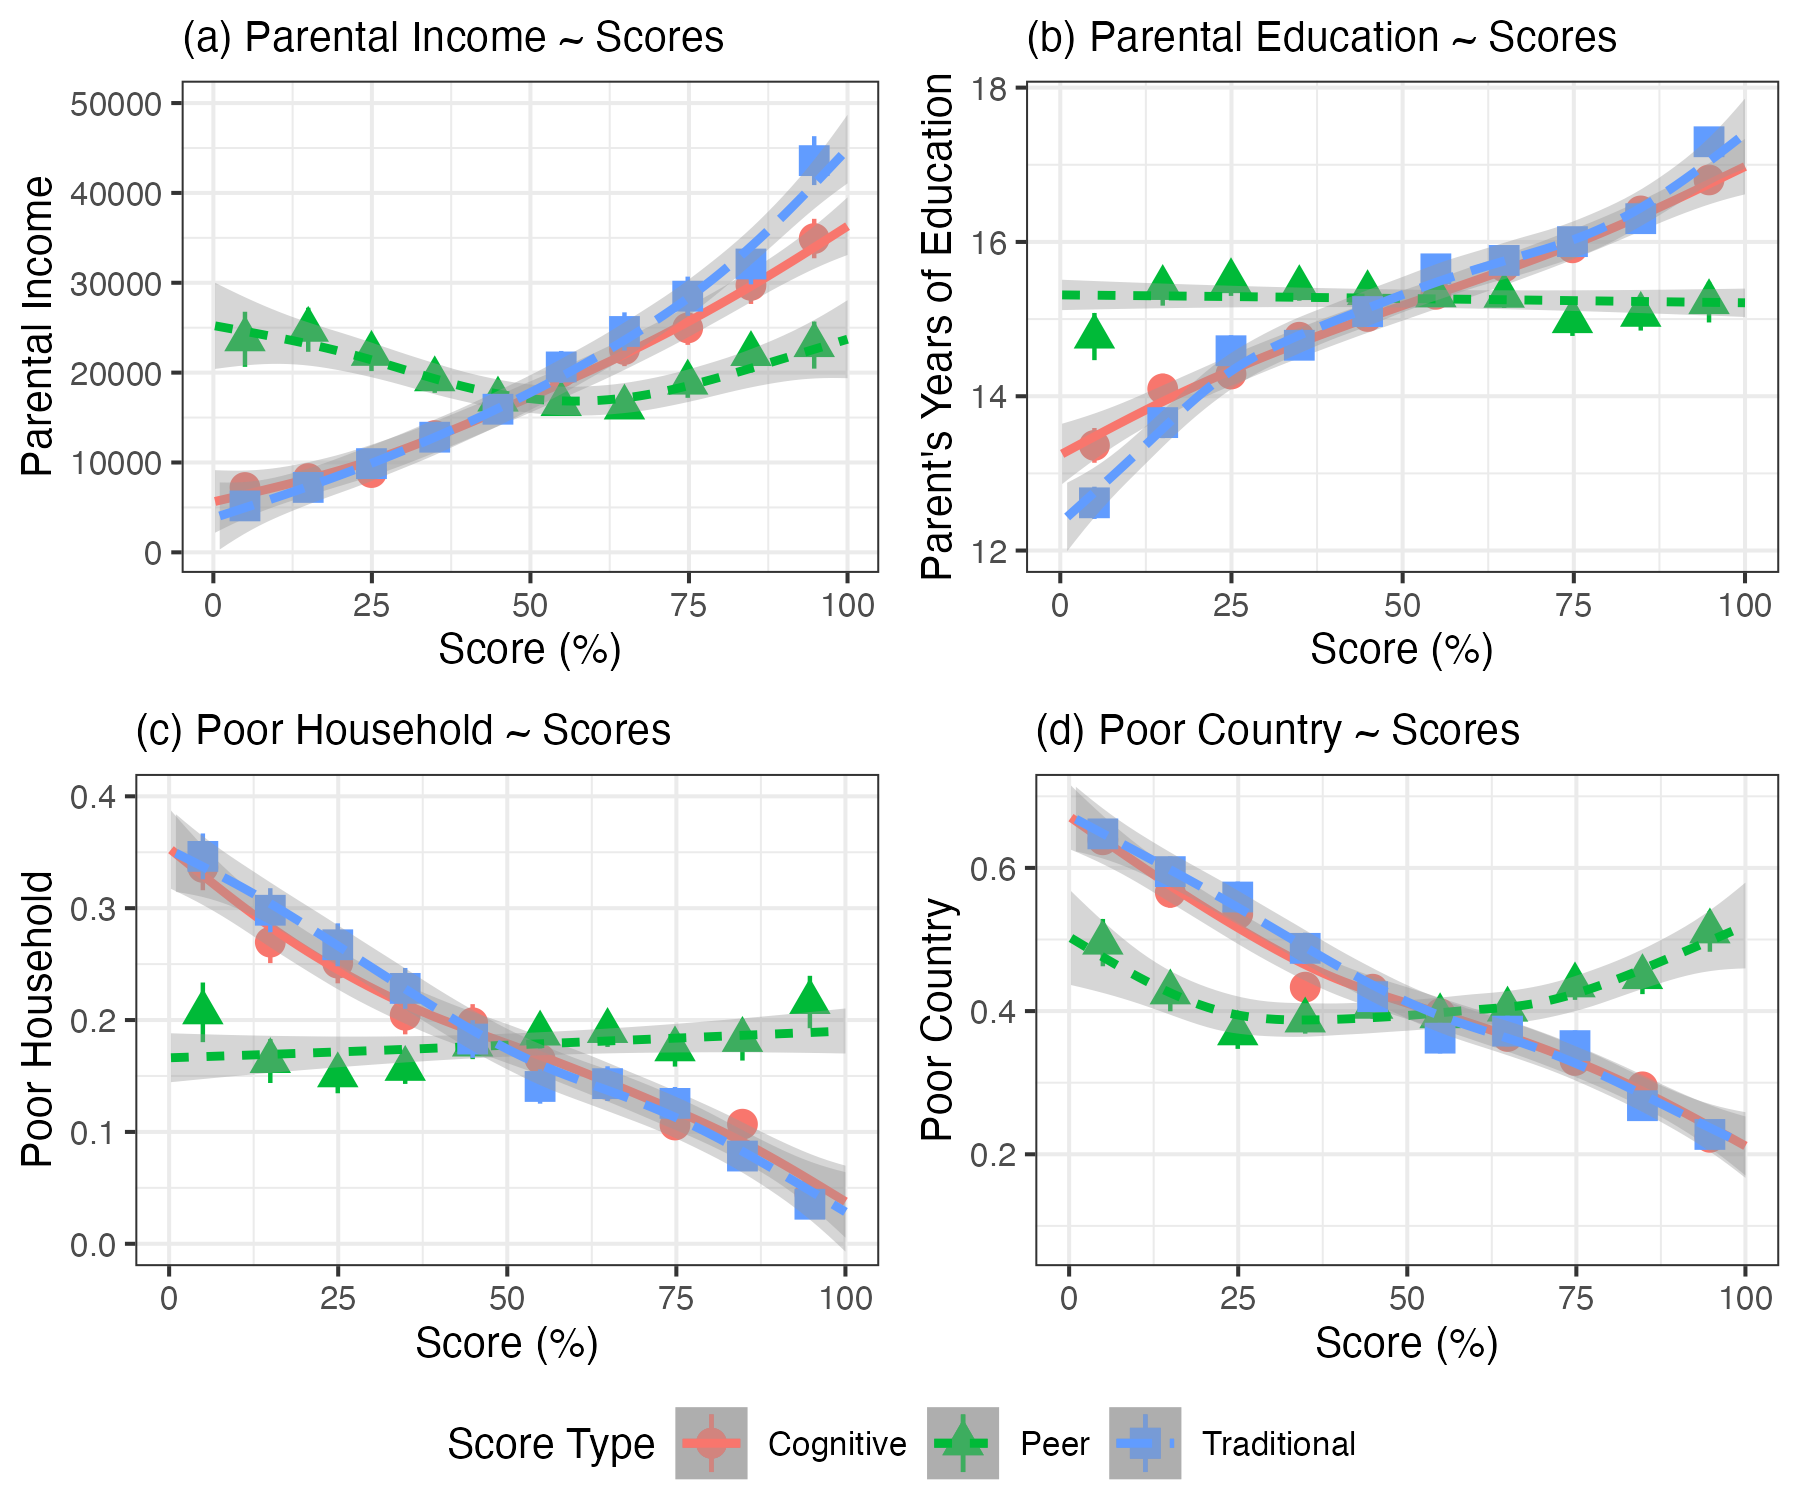
\includegraphics[width=\textwidth,height=\textheight,keepaspectratio]{spf/disadvantage_by_scores_full.png} 
    % \end{figure}
    
    % \newpage
    % \begin{figure}[!htb]
    % \centering
    %     \caption{This figure plots the average proportion female by deciles of cognitive, peer, and traditional scores for the cycle 1 cohort (Panel A) and all cohorts pooled together (Panel B). The cognitive score is the percentile of the candidate's IQ, the peer score is the percentile of the average peer assessment of each applicant video, and the traditional score is the average percentile of a candidate's IQ and project essay rating.}
    %     \label{fig:alt_female_cor}
    %     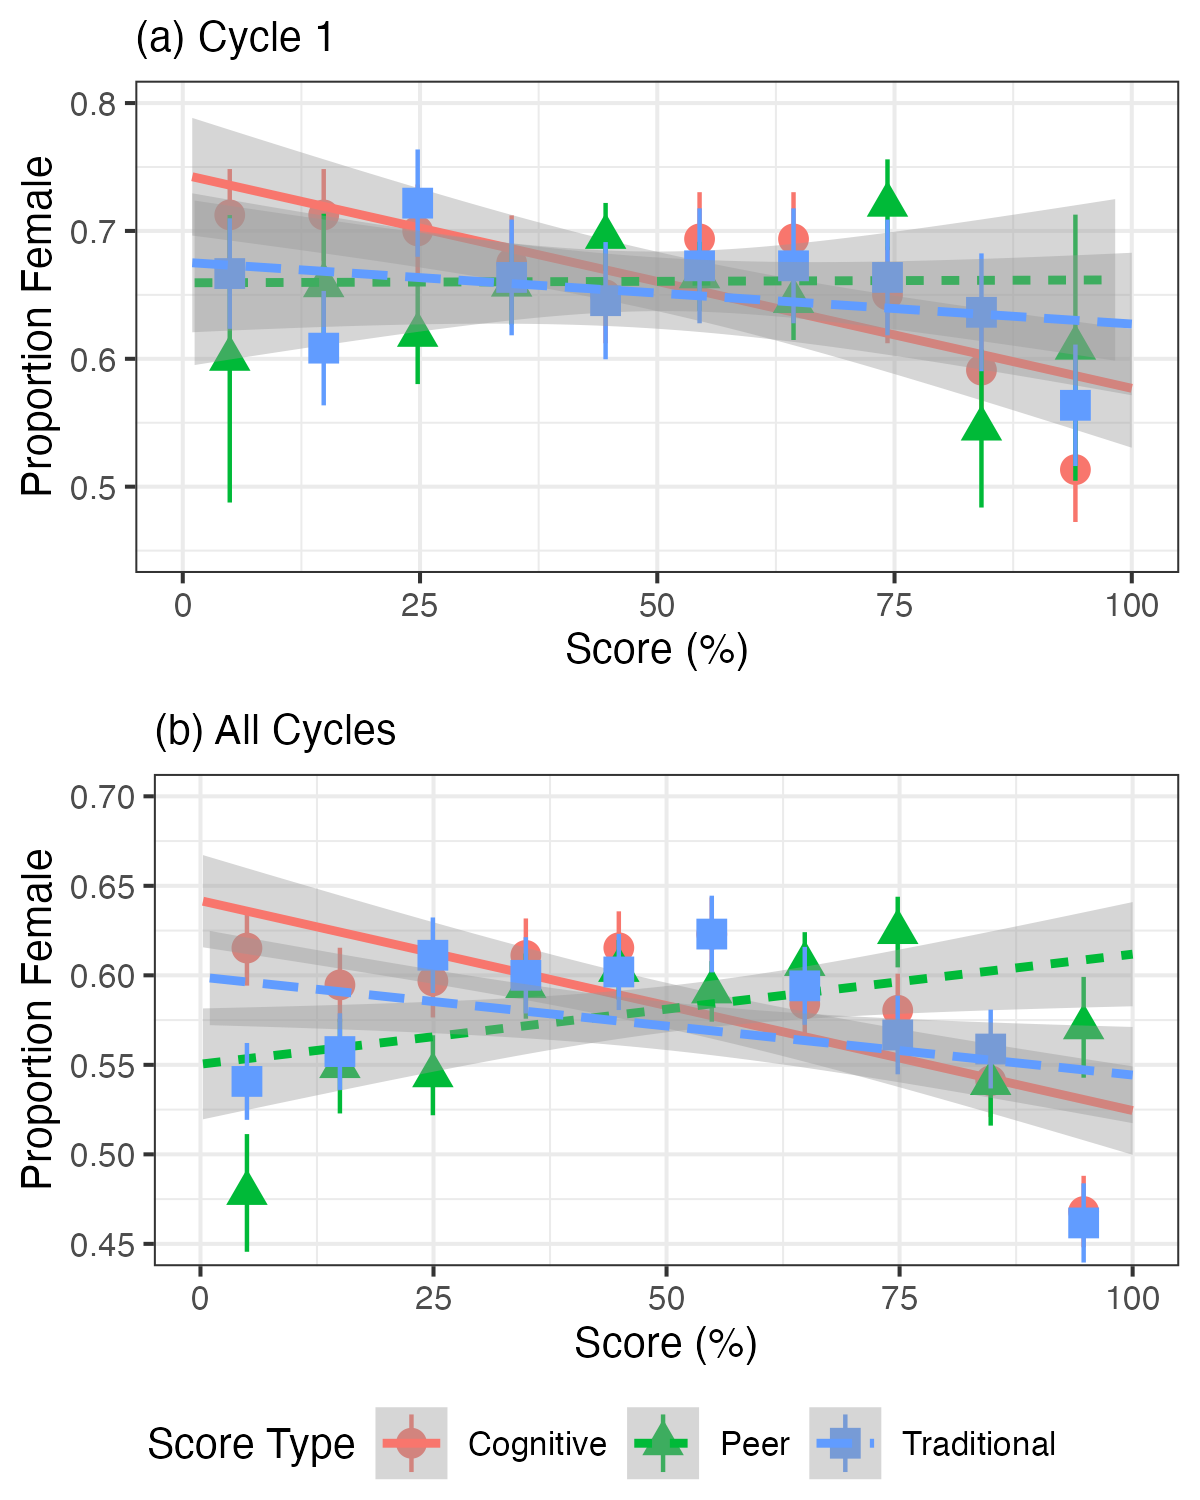
\includegraphics[width=.9\textwidth,height=\textheight,keepaspectratio]{spf/female_by_scores.png} 
    % \end{figure}
    
    
    % \newpage
    
    % \begin{table}[!htbp]
    %     \centering
    %     \caption{Summary Statistics: Risepplicants (Cycle 1). Raw data come from surveys completed by applicants. Data are pooled across all three application years. }
    %     \label{tab:c1_demo}
    % \begin{tabular}{@{\extracolsep{5pt}}lccccc} 
    % \\[-1.8ex]\hline 
    % \hline \\[-1.8ex] 
    % \emph{Panel A: Demographics} & \multicolumn{1}{c}{N} & \multicolumn{1}{c}{Mean} & \multicolumn{1}{c}{St. Dev.} & \multicolumn{1}{c}{Min} & \multicolumn{1}{c}{Max} \\ 
    % \hline \\[-1.8ex] 
    % Male & 1,591 & 0.33 & 0.47 & 0 & 1 \\ 
    % Age & 1,589 & 16.81 & 0.81 & 15 & 18 \\ 
    % Poor Country & 1,591 & 0.23 & 0.42 & 0 & 1 \\ 
    % Poor Household & 1,591 & 0.07 & 0.26 & 0 & 1 \\ 
    % Yrs of Parent Education & 1,591 & 15.61 & 4.73 & 0 & 20 \\ 
    % Mean Parent Income (\$) & 1,591 & 7,209 & 8,847 & 356 & 65,174 \\ 
    % \hline
    % & & & & & \\
    % \emph{Panel B: Global Region} & \multicolumn{1}{c}{N} & \multicolumn{1}{c}{Mean} & \multicolumn{1}{c}{St. Dev.} & \multicolumn{1}{c}{Min} & \multicolumn{1}{c}{Max} \\ 
    % \hline
    % Latin America & 1,591 & 0.46 & 0.50 & 0 & 1 \\ 
    % Canada/US/UK+ & 1,591 & 0.15 & 0.36 & 0 & 1 \\ 
    % Middle East & 1,591 & 0.11 & 0.32 & 0 & 1 \\ 
    % Sub-Saharan Africa & 1,591 & 0.09 & 0.29 & 0 & 1 \\ 
    % India & 1,591 & 0.06 & 0.23 & 0 & 1 \\ 
    % Western Europe & 1,591 & 0.05 & 0.22 & 0 & 1 \\ 
    % East Asia & 1,591 & 0.04 & 0.19 & 0 & 1 \\ 
    % Caribbean/Pacific Islands & 1,591 & 0.003 & 0.05 & 0 & 1 \\ 
    % Eastern Europe & 1,591 & 0.00 & 0.00 & 0 & 0 \\ 
    % \hline \hline \\[-1.8ex] 
    % \end{tabular} 
    % \end{table} 
    
    % \hfill

% \begin{table}[!htb]
% % to-do: add back details in this table.
% \caption{Key Measures and Components. This table provides an overview of the key measures used in this paper. Column 1 gives the name of the measure as it is used throughout the paper. Column 2 describes the attribute the measure is supposed to capture and the summarizes the measure construction process. Column 3 contains the number of items used to generate the measure. Column 4 contains the scale of the answers used for each of the items. Column 5 lists sample items to give a sense of the type of items used to construct the measure. More details about the data construction can be provided by the authors if requested.}
% \label{tab:measure_details}
% \end{table}

    
    % \begin{table}[!htb]
    % \caption{Key Measures and Components. This table provides an overview of the key measures used in this paper. Column 1 gives the name of the measure as it is used throughout the paper. Column 2 describes the attribute the measure is supposed to capture and the summarizes the measure construction process. Column 3 contains the number of items used to generate the measure. Column 4 contains the scale of the answers used for each of the items. Column 5 lists sample items to give a sense of the type of items used to construct the measure. More details about the data construction can be provided by the authors if requested.}
    % \begin{tabular}{1.6\textwidth}{c | p{2cm} | c | l | p{2cm} }
    % \toprule
    % Measure Name & Description & Number of Items & Item Scale(s) & Sample Item(s)   \\ 
    % \hline
    % \hspace{3pt} Project Quality \\ (``Talent") & The programme's primary talent measure constructed from taking the percentilized sum of experts' project \emph{Effectiveness} and project \emph{Impressiveness} ratings.  & 2 & Likert: 1-15 & 1. The [Project] was an effective response to the [Problem] 2. The [Project] is impressive given their age and experience \\
    % \hline
    % \hspace{3pt} Cognitive Ability & A 15 item version of the The International Cognitive Ability Resource (ICAR) Intelligence Test. Scores are constructed using Bayesian estimation of a 2 parameter Item Response Theory (IRT) model following \citeA{burkner2021bayesian}. & 15 & Mult. Choice: 6-8 (options) & See Figure \ref{fig:icar_items} for example items of each type\\
    % \hline
    % \hspace{3pt} Traditional Score & A measure of talent meant to mimic traditional selection methods by relying solely on test scores (i.e. ICAR) and ratings of the written project summary essay. The score is constructed by taking the average of the sum of percentiles of ICAR and essay ratings. & 13 & 1. Likert: 1-15 2. Mult. Choice: 6-8 & 1. See Figure \ref{fig:icar_items} for example items from ICAR 2. The [Project] was an effective response to the [Problem] \\
    % \hline
    % \hspace{3pt} Peer Score & Average percentile of peer scores given for each of the video essays and project videos. & 12 & Likert: 1-7  & 1. How likely is it that this person will dedicate part of their life to solving this problem? 2. The [Project] was an effective response to the [Problem] \\
    % \hline
    % \bottomrule
    % \end{tabular}
    % \label{tab:measure_details}
    % \end{table}
    \hfill